% ---------------------------------------------------------------
% 5. Processo de decisão e explicação
% ---------------------------------------------------------------
\chapter{Processo de decisão e explicação}\label{cap:decisao}

\section{Fluxograma de decisão}\label{sec:fluxograma}

A Figura 4 representa o ciclo de raciocínio, repetido a cada 100 ms. Em cada ciclo, as regras são avaliadas por fases, cuja ordem é imposta por uma meta-regra. Na fase de perceção, as leituras dos sensores são convertidas em factos que descrevem a situação, como «peão na passadeira» ou «TTC baixo». Na fase de decisão, cada regra cujas condições se verificam não executa diretamente uma ação, apenas a propõe. Se nenhuma regra de decisão for ativada, a fase de recurso garante que existe sempre uma ação como, por exemplo, manter a velocidade ou retomar a marcha. No fim do ciclo, todas as propostas são comparadas e é escolhida a ação a executar. Como a escolha é feita apenas no fim, depois de recolhidas todas as propostas, a ordem pela qual as regras disparam não altera o resultado. Neste sentido, a ação final é composta por duas decisões independentes: a decisão de velocidade (acelerar, travar ou parar) e a decisão de via (manter, mudar ou regressar à direita).

Na decisão de velocidade, uma proposta de emergência ou de paragem obrigatória (prioridade 60 ou superior) sobrepõe-se a todas as outras. Ganha a de maior prioridade e, em caso de empate, a de menor velocidade. Se outra regra exigir uma velocidade ainda mais baixa, mantém-se a ação escolhida, mas com essa velocidade. Abaixo desse nível, as propostas de prioridade 50, 40 e 20 funcionam como limites máximos de velocidade. Como o veículo tem de os respeitar todos ao mesmo tempo, adota-se o mais baixo; as propostas de prioridade 30 e 10 dão apenas a velocidade de base quando nenhum teto é inferior, pelo que nenhuma regra consegue levar o veículo acima do limite legal por ter uma prioridade maior (Figura 5). No que diz respeito à decisão de via (Figura 6), ganha a proposta de maior prioridade e, em empate, regressar à direita vence mudar de via, que vence manter a via. No entanto, uma travagem de emergência nunca dá origem a uma avaliação de manobra: as duas decisões são tomadas em separado e, em caso de conflito, a travagem prevalece. No fim do ciclo, a decisão e o destino de todas as propostas ficam registados e são enviados para a interface, que é o último passo da Figura 4.

\begin{figure}[p]
\centering
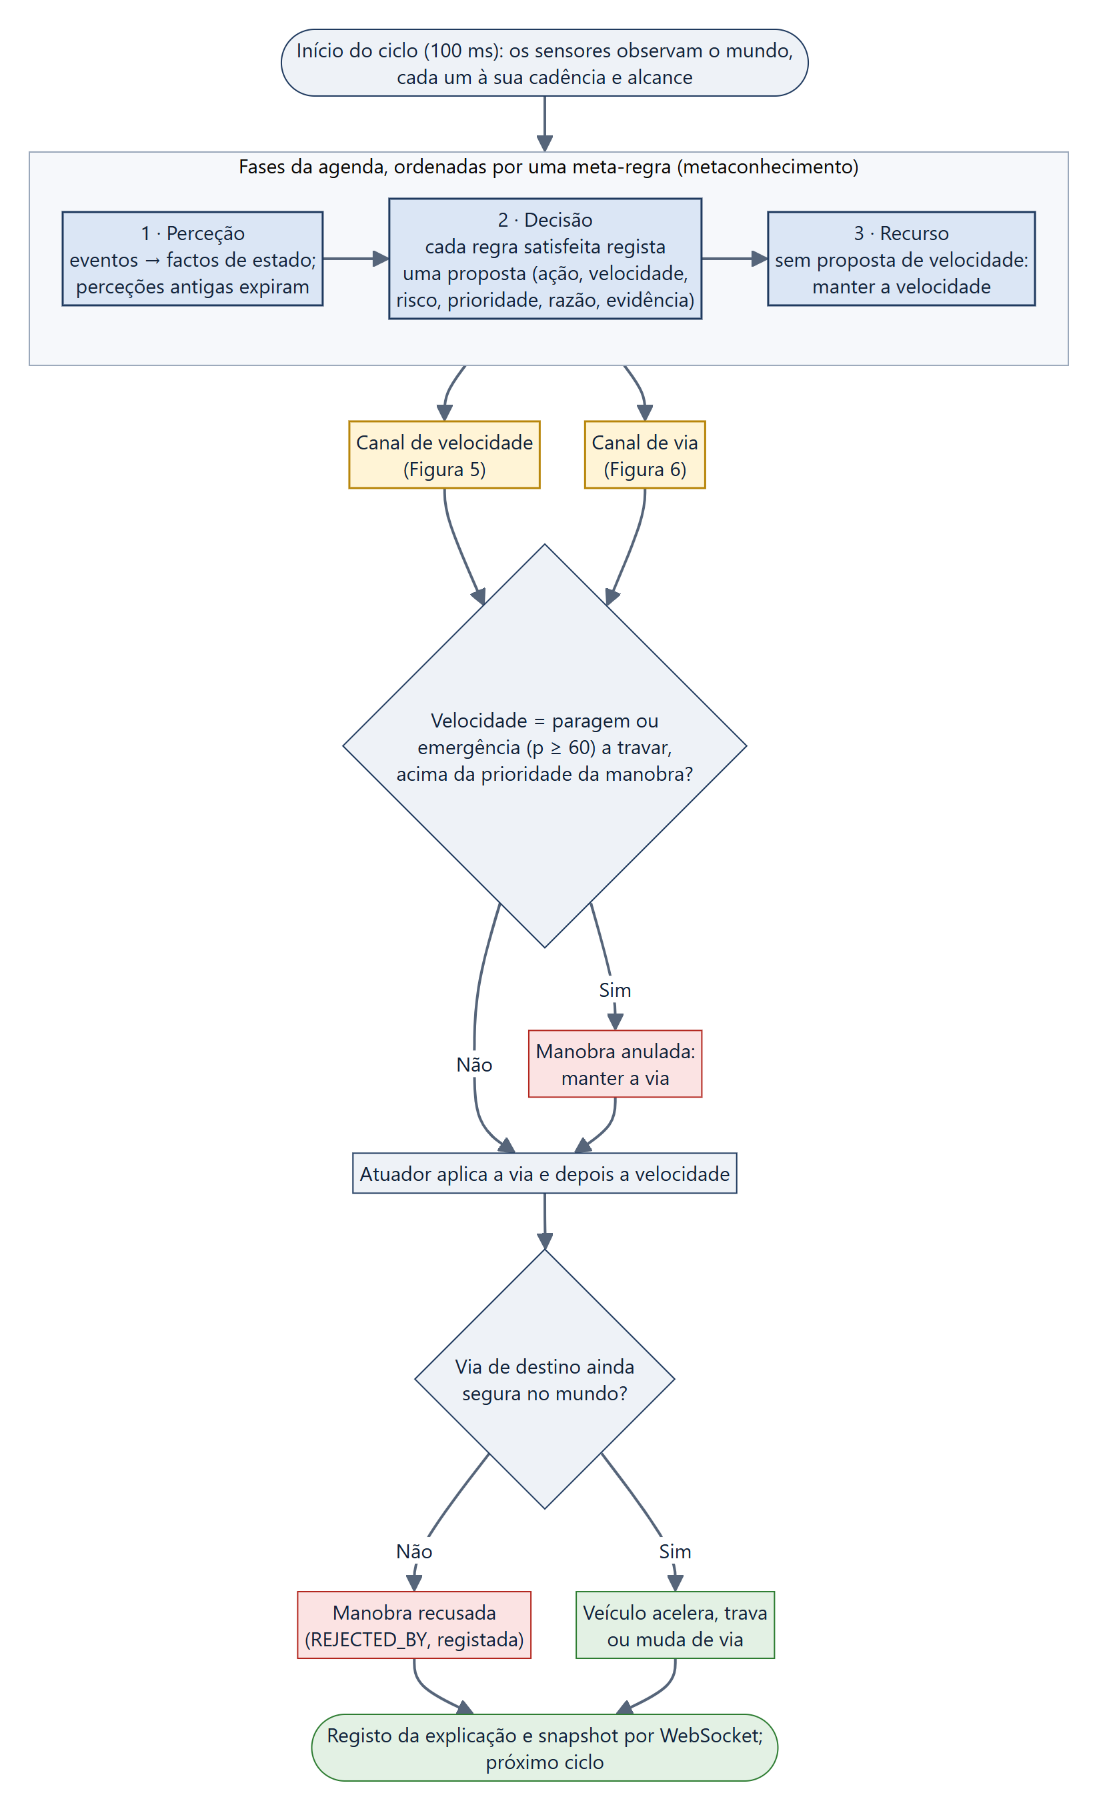
\includegraphics[width=\textwidth,height=0.92\textheight,keepaspectratio]{figuras/ciclo_decisao.png}
\caption{Fluxograma de inferência e decisão em cada ciclo de 100 ms}
\label{fig:ciclo-decisao}
\end{figure}

As Figuras 5 e 6 detalham, para cada canal, as perguntas pela ordem de importância. A travagem de emergência está no canal de velocidade e nunca passa pela pergunta ``a manobra é permitida?».

\begin{figure}[p]
\centering
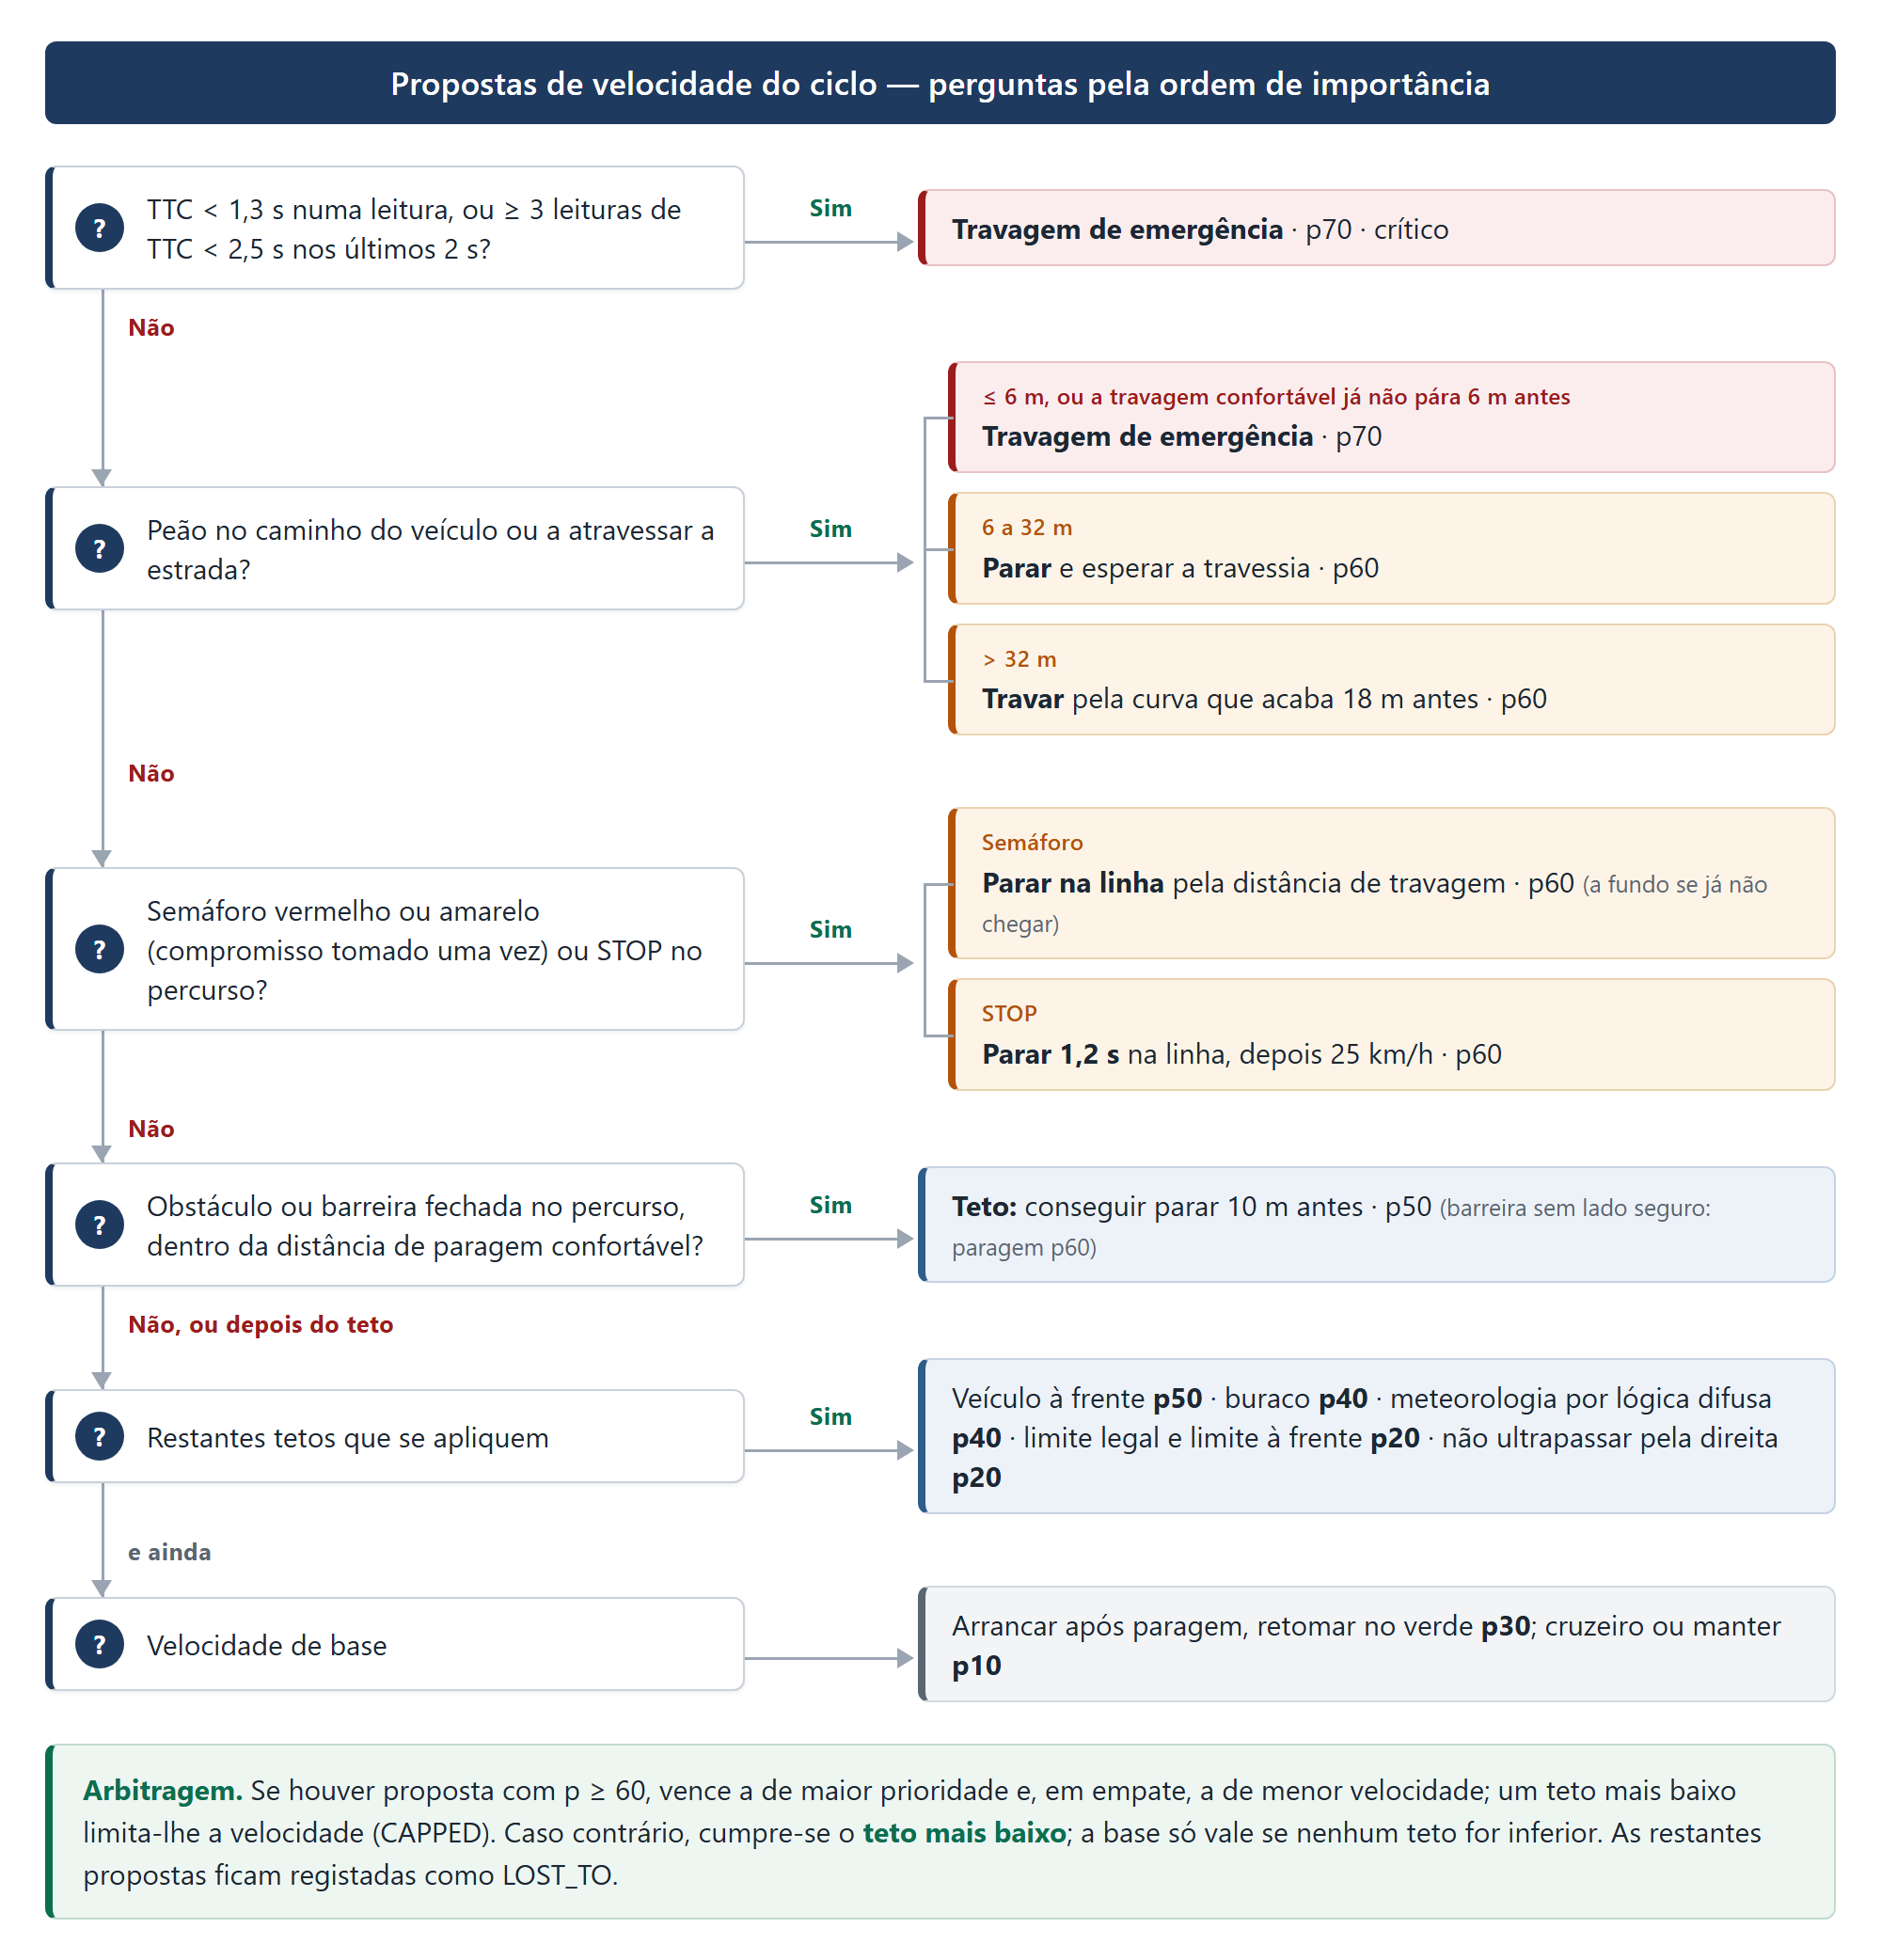
\includegraphics[width=\textwidth,height=0.92\textheight,keepaspectratio]{figuras/canal_velocidade.png}
\caption{Canal de velocidade: perguntas pela ordem de importância e arbitragem}
\label{fig:canal-velocidade}
\end{figure}

\begin{figure}[p]
\centering
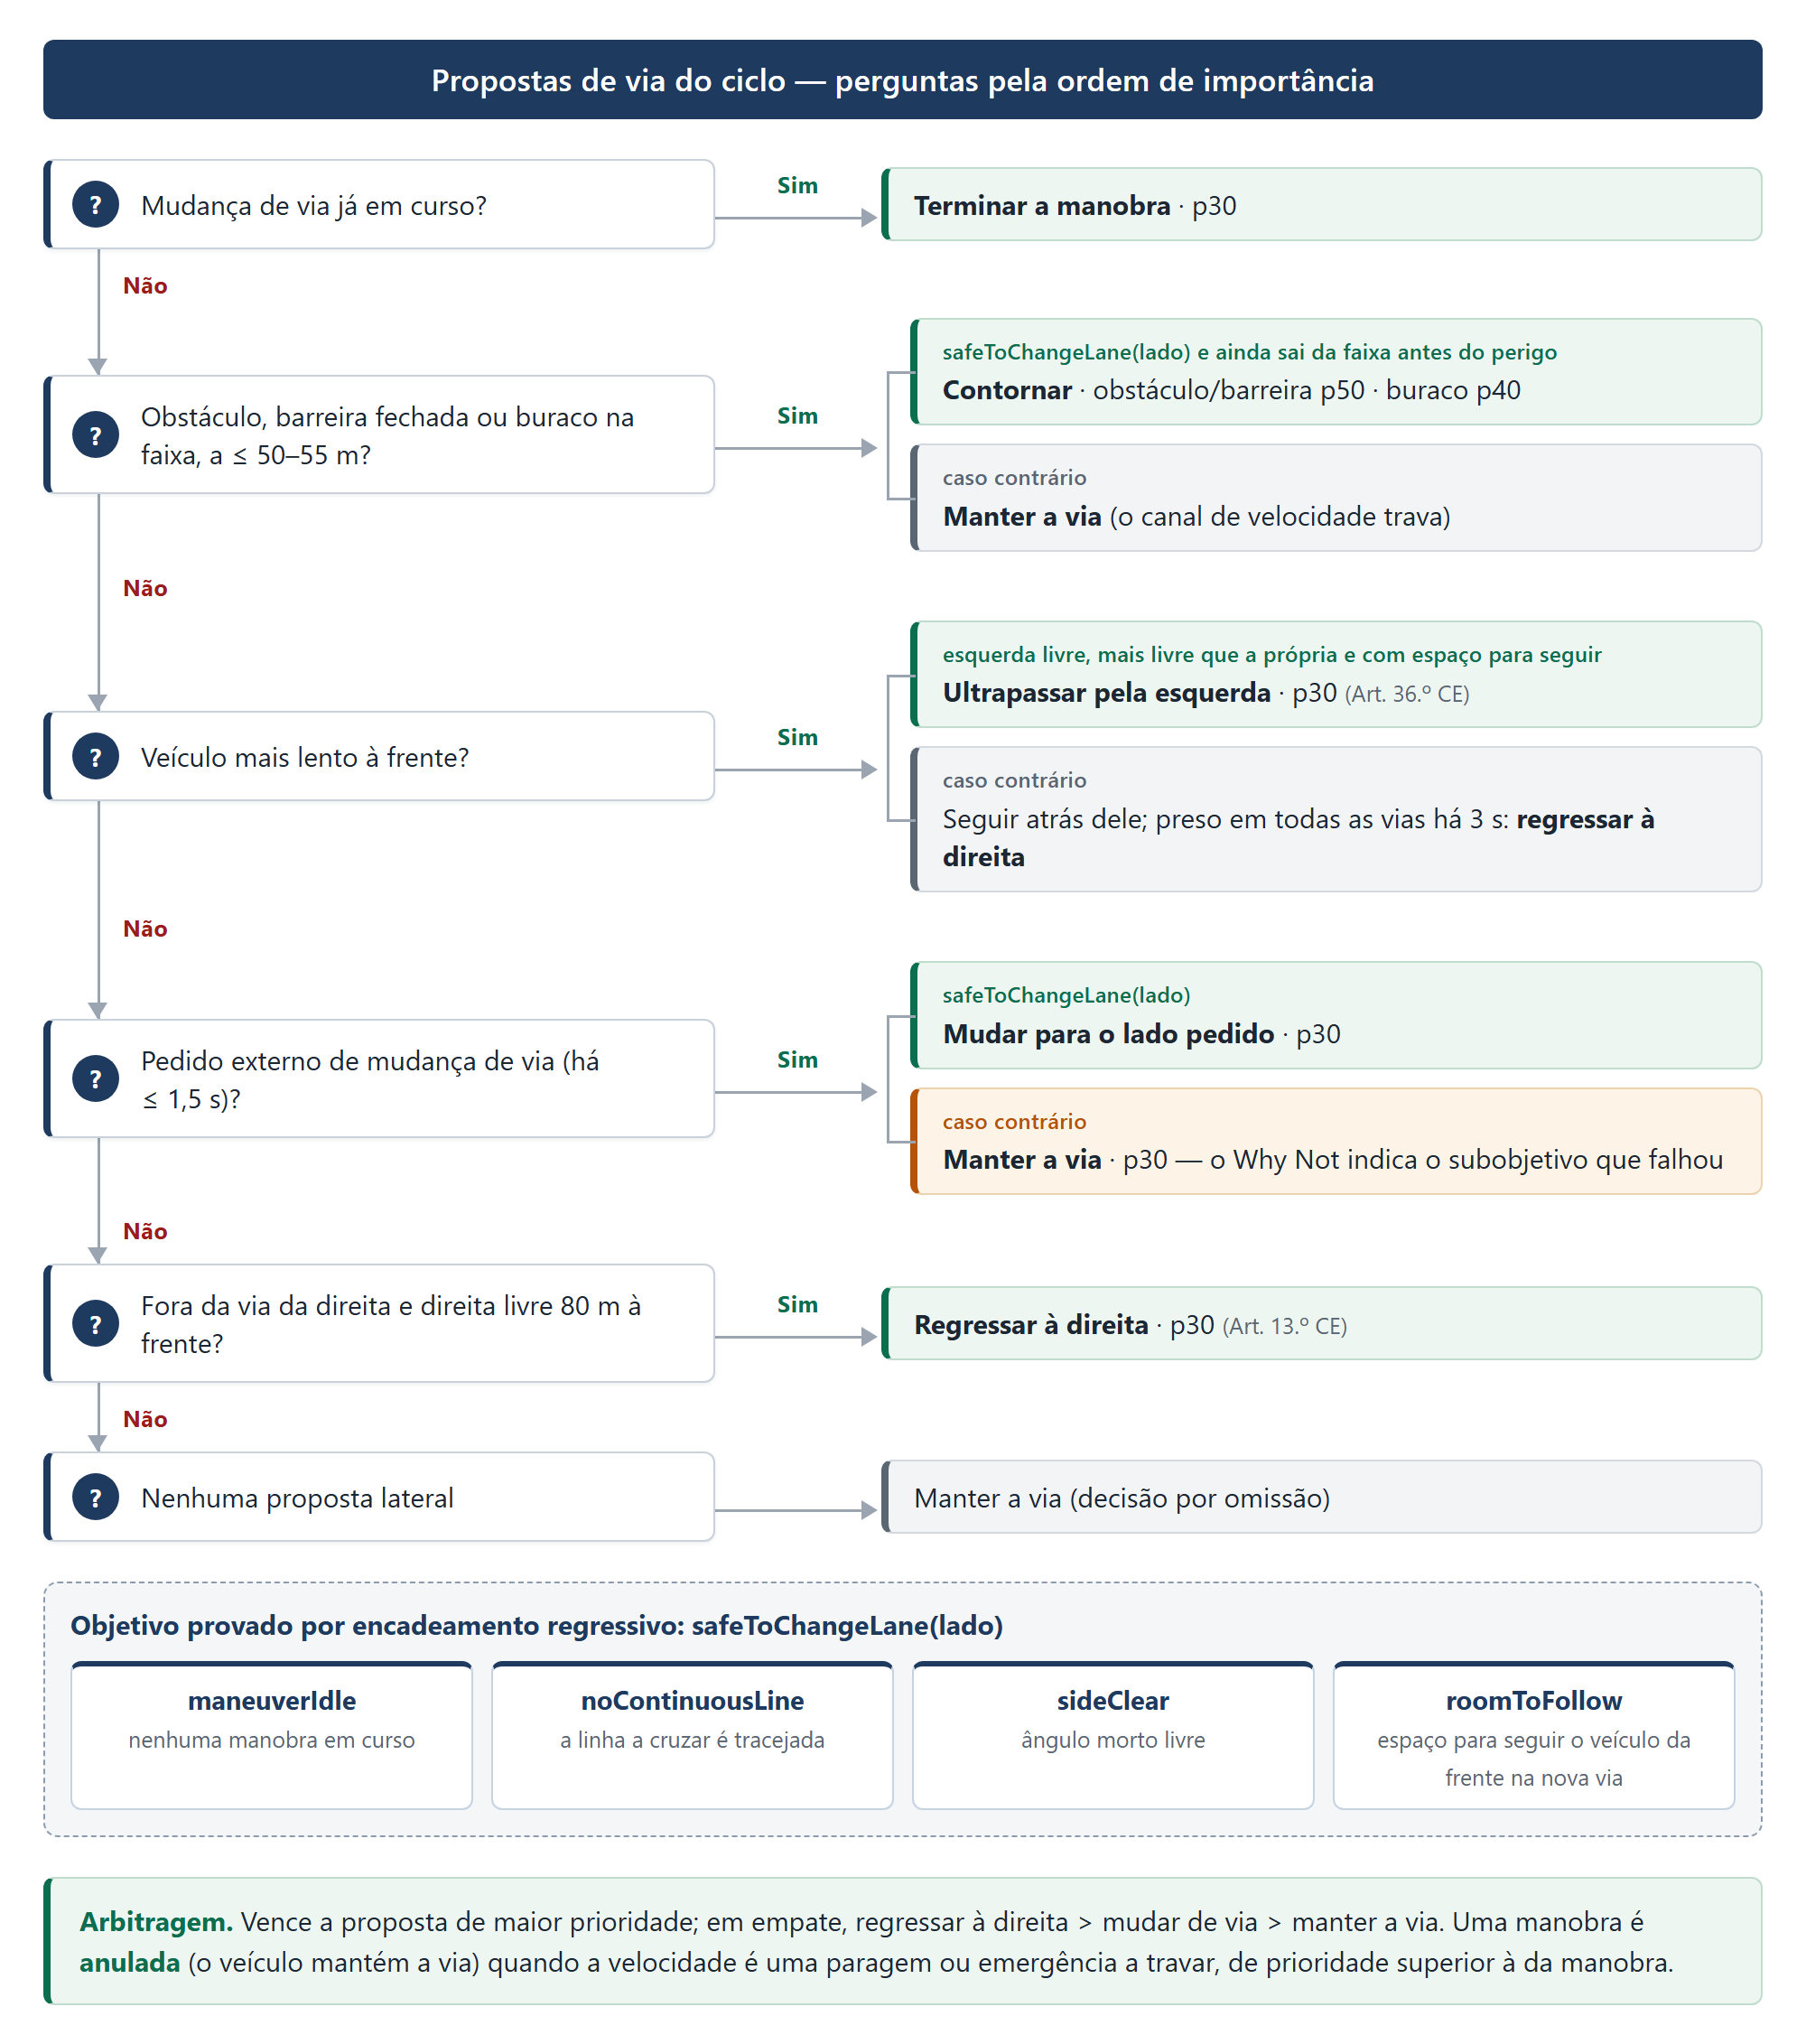
\includegraphics[width=\textwidth,height=0.92\textheight,keepaspectratio]{figuras/canal_via.png}
\caption{Canal de via e objetivo provado por encadeamento regressivo}
\label{fig:canal-via}
\end{figure}

\FloatBarrier
\section{Fluxograma completo}\label{sec:fluxograma-completo}

As Figuras 4 a 6 resumem o processo de decisão. A Figura 7 apresenta-o por inteiro: 49 perguntas e 43 ações, repetidas em cada ciclo de 100 ms. Para facilitar a leitura, o fluxograma foi dividido em sete zonas, cada uma com uma cor. As zonas A a E formam o canal de velocidade, as zonas F e G o canal de via, e a zona G termina com a atuação. Cada zona é ampliada numa figura própria (Figuras 8 a 14). No canto de cada ampliação, um pequeno mapa indica a zona em que o leitor se encontra, e as caixas tracejadas indicam de onde vem e para onde segue o fluxo. A versão vetorial do fluxograma completo, que pode ser ampliada sem perda de qualidade, é referida no Anexo B.

Este fluxograma deve ser lido como uma ordem de importância e não como uma sequência de execução. No Drools, todas as regras cujas condições se verificam disparam no mesmo ciclo e registam a sua proposta. A arbitragem descrita na Secção 5.1 escolhe depois a proposta vencedora. Como essa escolha segue as mesmas prioridades, o resultado é igual ao de percorrer o fluxograma de cima para baixo. Os hexágonos representam perguntas, os retângulos verdes representam ações e os vermelhos representam travagens fortes ou manobras canceladas.

\begin{sidewaysfigure}
\centering
\includegraphics[width=\textheight,height=0.92\textwidth,keepaspectratio]{figuras/fluxograma/fluxograma_completo.pdf}
\caption{Fluxograma completo do processo de decisão, dividido em zonas}
\label{fig:fluxo-completo}
\end{sidewaysfigure}

\begin{sidewaysfigure}
\begin{minipage}{\linewidth}
\noindent\textbf{Zona A -- Emergência e peões (\cref{fig:zonaA}).} É a primeira zona, porque trata
as situações em que está em causa uma colisão. Uma única leitura de TTC inferior a 1,3 s, ou três
leituras inferiores a 2,5 s nos últimos 2 s, origina uma travagem de emergência com luzes de
emergência (prioridade 70). Se houver um peão no caminho do veículo, a resposta depende da
distância. A 6 m ou menos, ou quando a travagem confortável já não permite parar 6 m antes, trava a
fundo. Entre 6 e 32 m, pára e espera que o peão termine a travessia. A mais de 32 m, abranda para
conseguir parar 18 m antes. Um obstáculo grave a 8 m ou menos, na via em que o veículo circula,
também origina uma emergência. A travagem de emergência termina diretamente na decisão de
velocidade e nunca passa por uma avaliação de manobra.
\end{minipage}

\vspace{4mm}
\centering
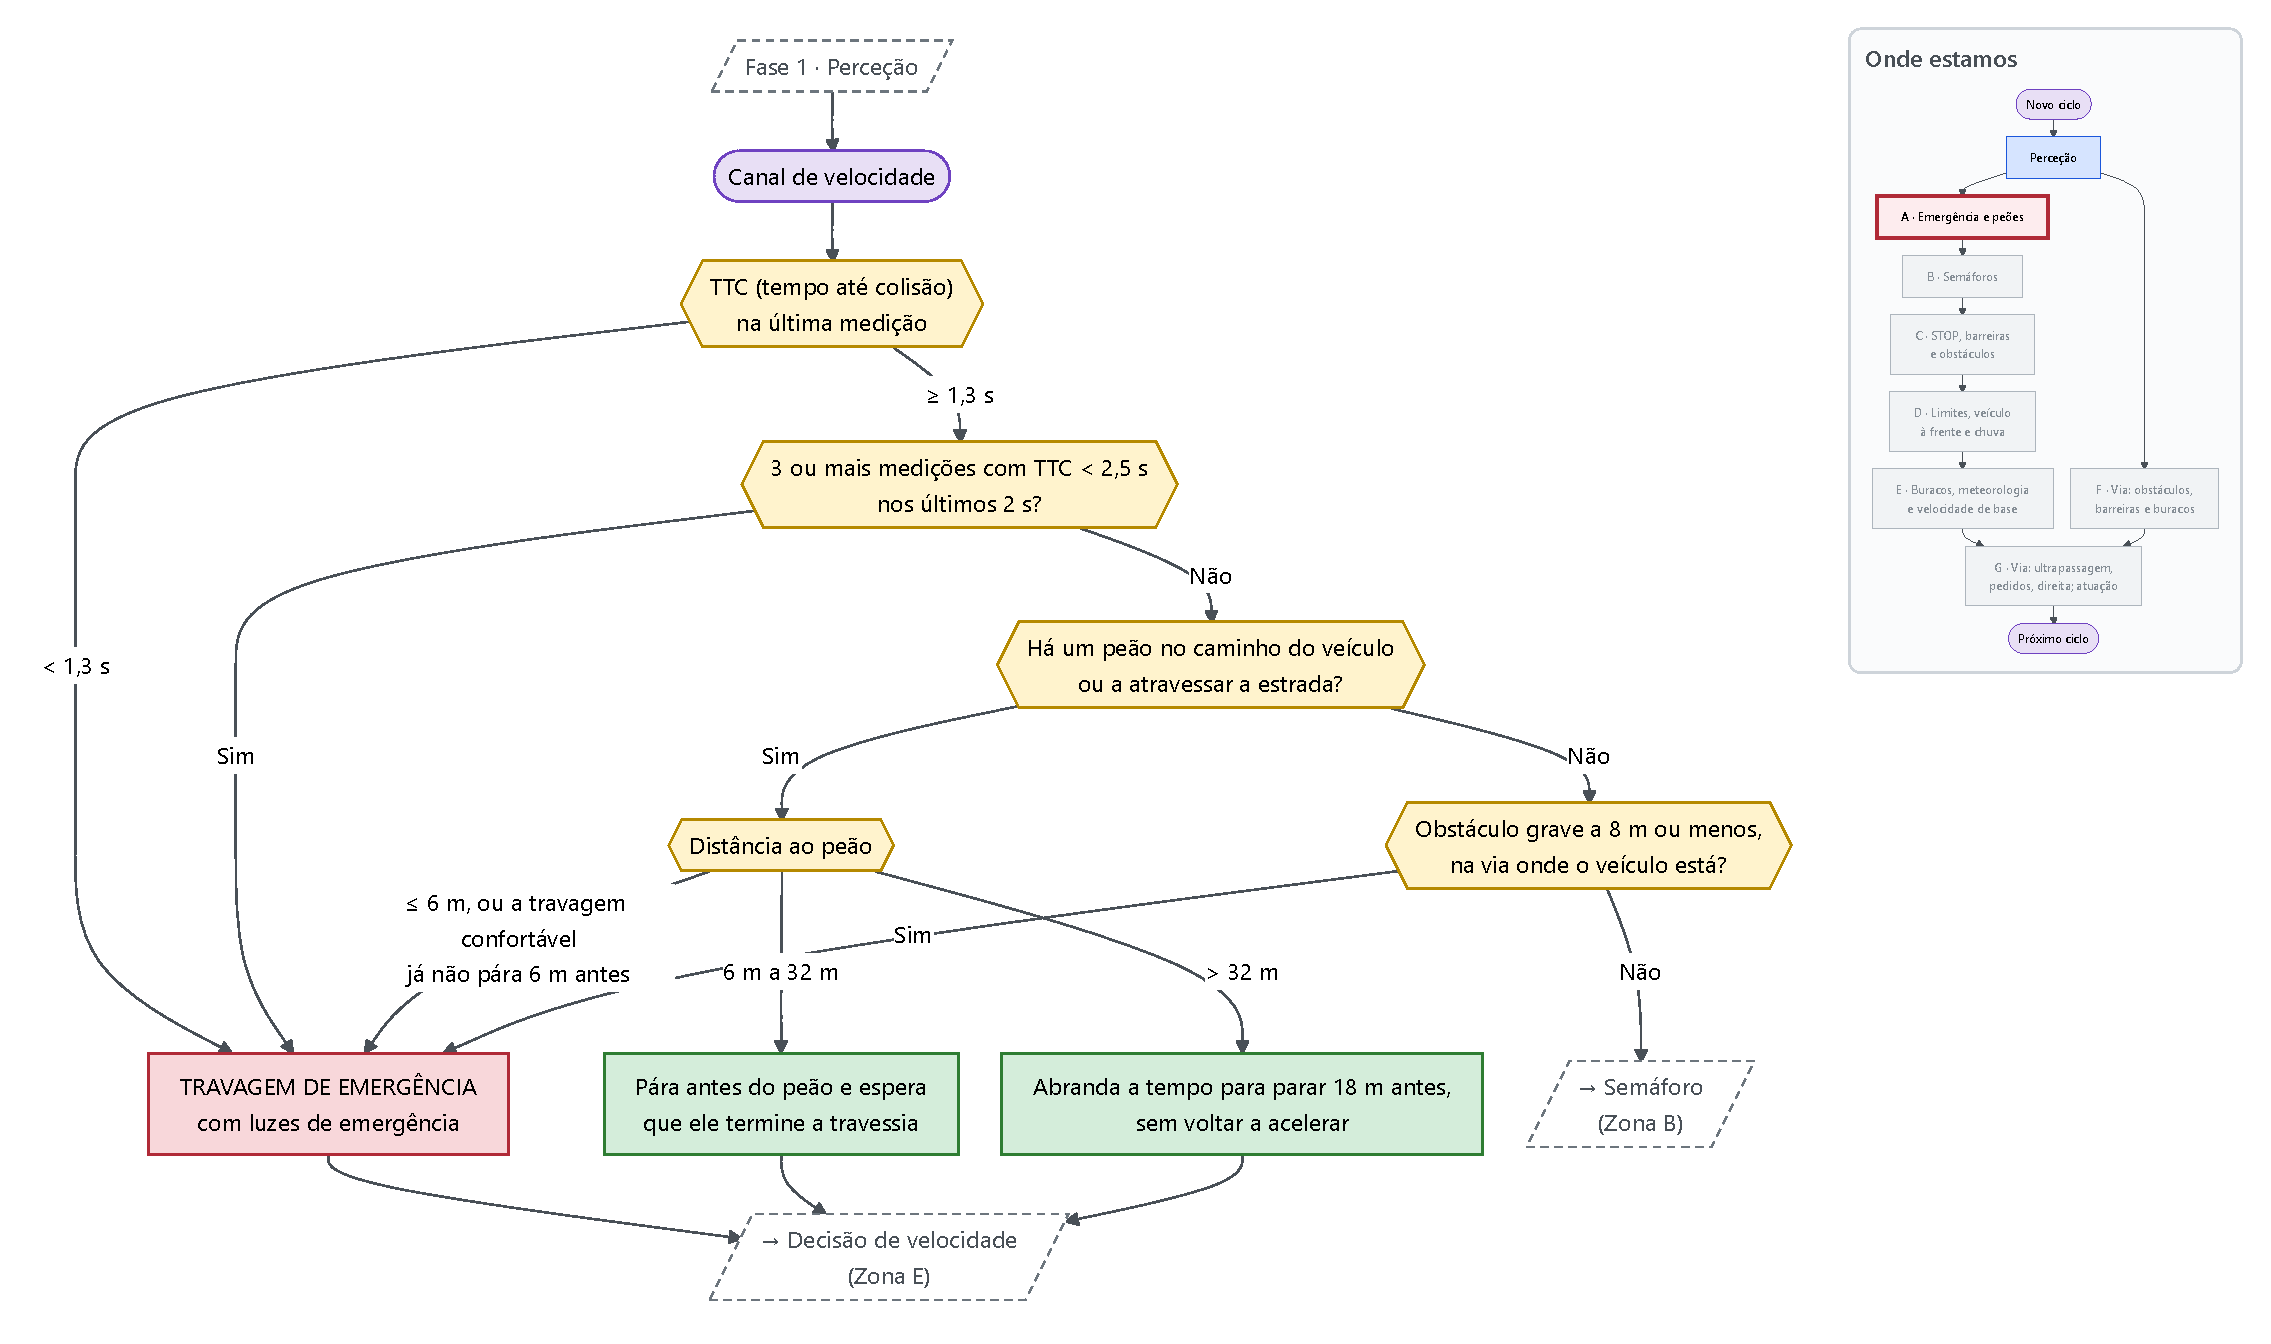
\includegraphics[width=\textheight,height=0.62\textwidth,keepaspectratio]{figuras/fluxograma/zona_A.pdf}
\caption{Zona A: emergência e peões}
\label{fig:zonaA}
\end{sidewaysfigure}

\begin{sidewaysfigure}
\begin{minipage}{\linewidth}
\noindent\textbf{Zona B -- Semáforos (\cref{fig:zonaB}).} Perante um semáforo vermelho, o veículo
compara a distância à linha com a distância de que precisa para parar: 0,5 s de reação, mais a
travagem, mais 18 m. Se estiver longe, continua. Se estiver na zona de transição, deixa de acelerar.
Se já estiver dentro da distância de travagem, trava com conforto (2,8 m/s²) e pára na linha, ou
trava a fundo quando a travagem confortável o levaria mais de 2 m para lá da linha. No amarelo, a
decisão de parar ou prosseguir é tomada uma única vez, para evitar que o veículo hesite e trave a
meio do cruzamento. No verde, o veículo segue ou volta a arrancar.
\end{minipage}

\vspace{4mm}
\centering
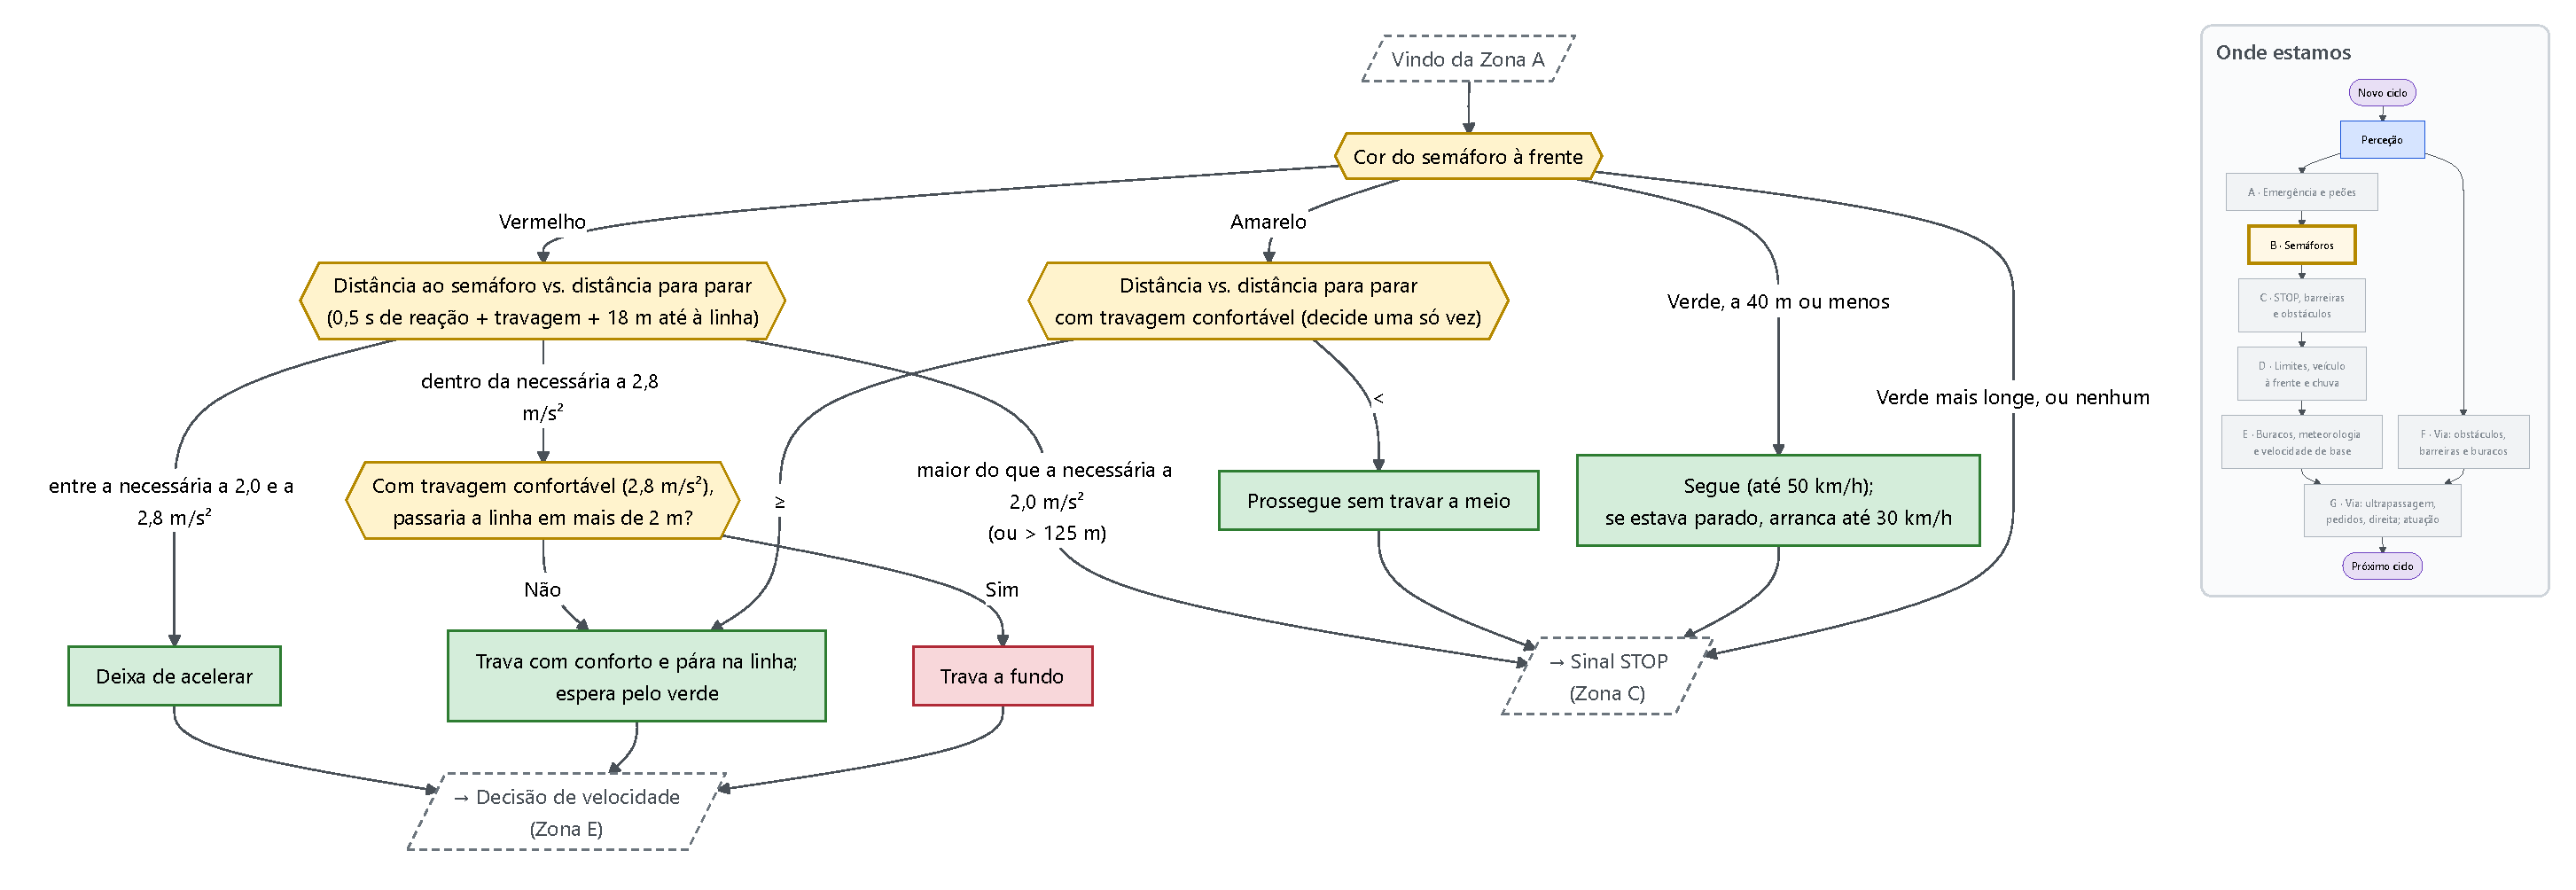
\includegraphics[width=\textheight,height=0.66\textwidth,keepaspectratio]{figuras/fluxograma/zona_B.pdf}
\caption{Zona B: semáforos}
\label{fig:zonaB}
\end{sidewaysfigure}

\begin{sidewaysfigure}
\begin{minipage}{\linewidth}
\noindent\textbf{Zona C -- STOP, barreiras e obstáculos (\cref{fig:zonaC}).} No sinal STOP, o
veículo pára na linha e só avança, a 25 km/h, depois de estar parado pelo menos 1,2 s, o que
garante a paragem completa exigida pelo Código da Estrada. Perante uma barreira fechada ou um
obstáculo dentro da distância de paragem confortável, o veículo trava para conseguir parar 10 m
antes. No caso da barreira, se for seguro mudar de via, essa travagem dura apenas até a mudança o
tirar do caminho. Se for preciso travar a mais de 3,1 m/s², a travagem passa a ser a fundo.
\end{minipage}

\vspace{4mm}
\centering
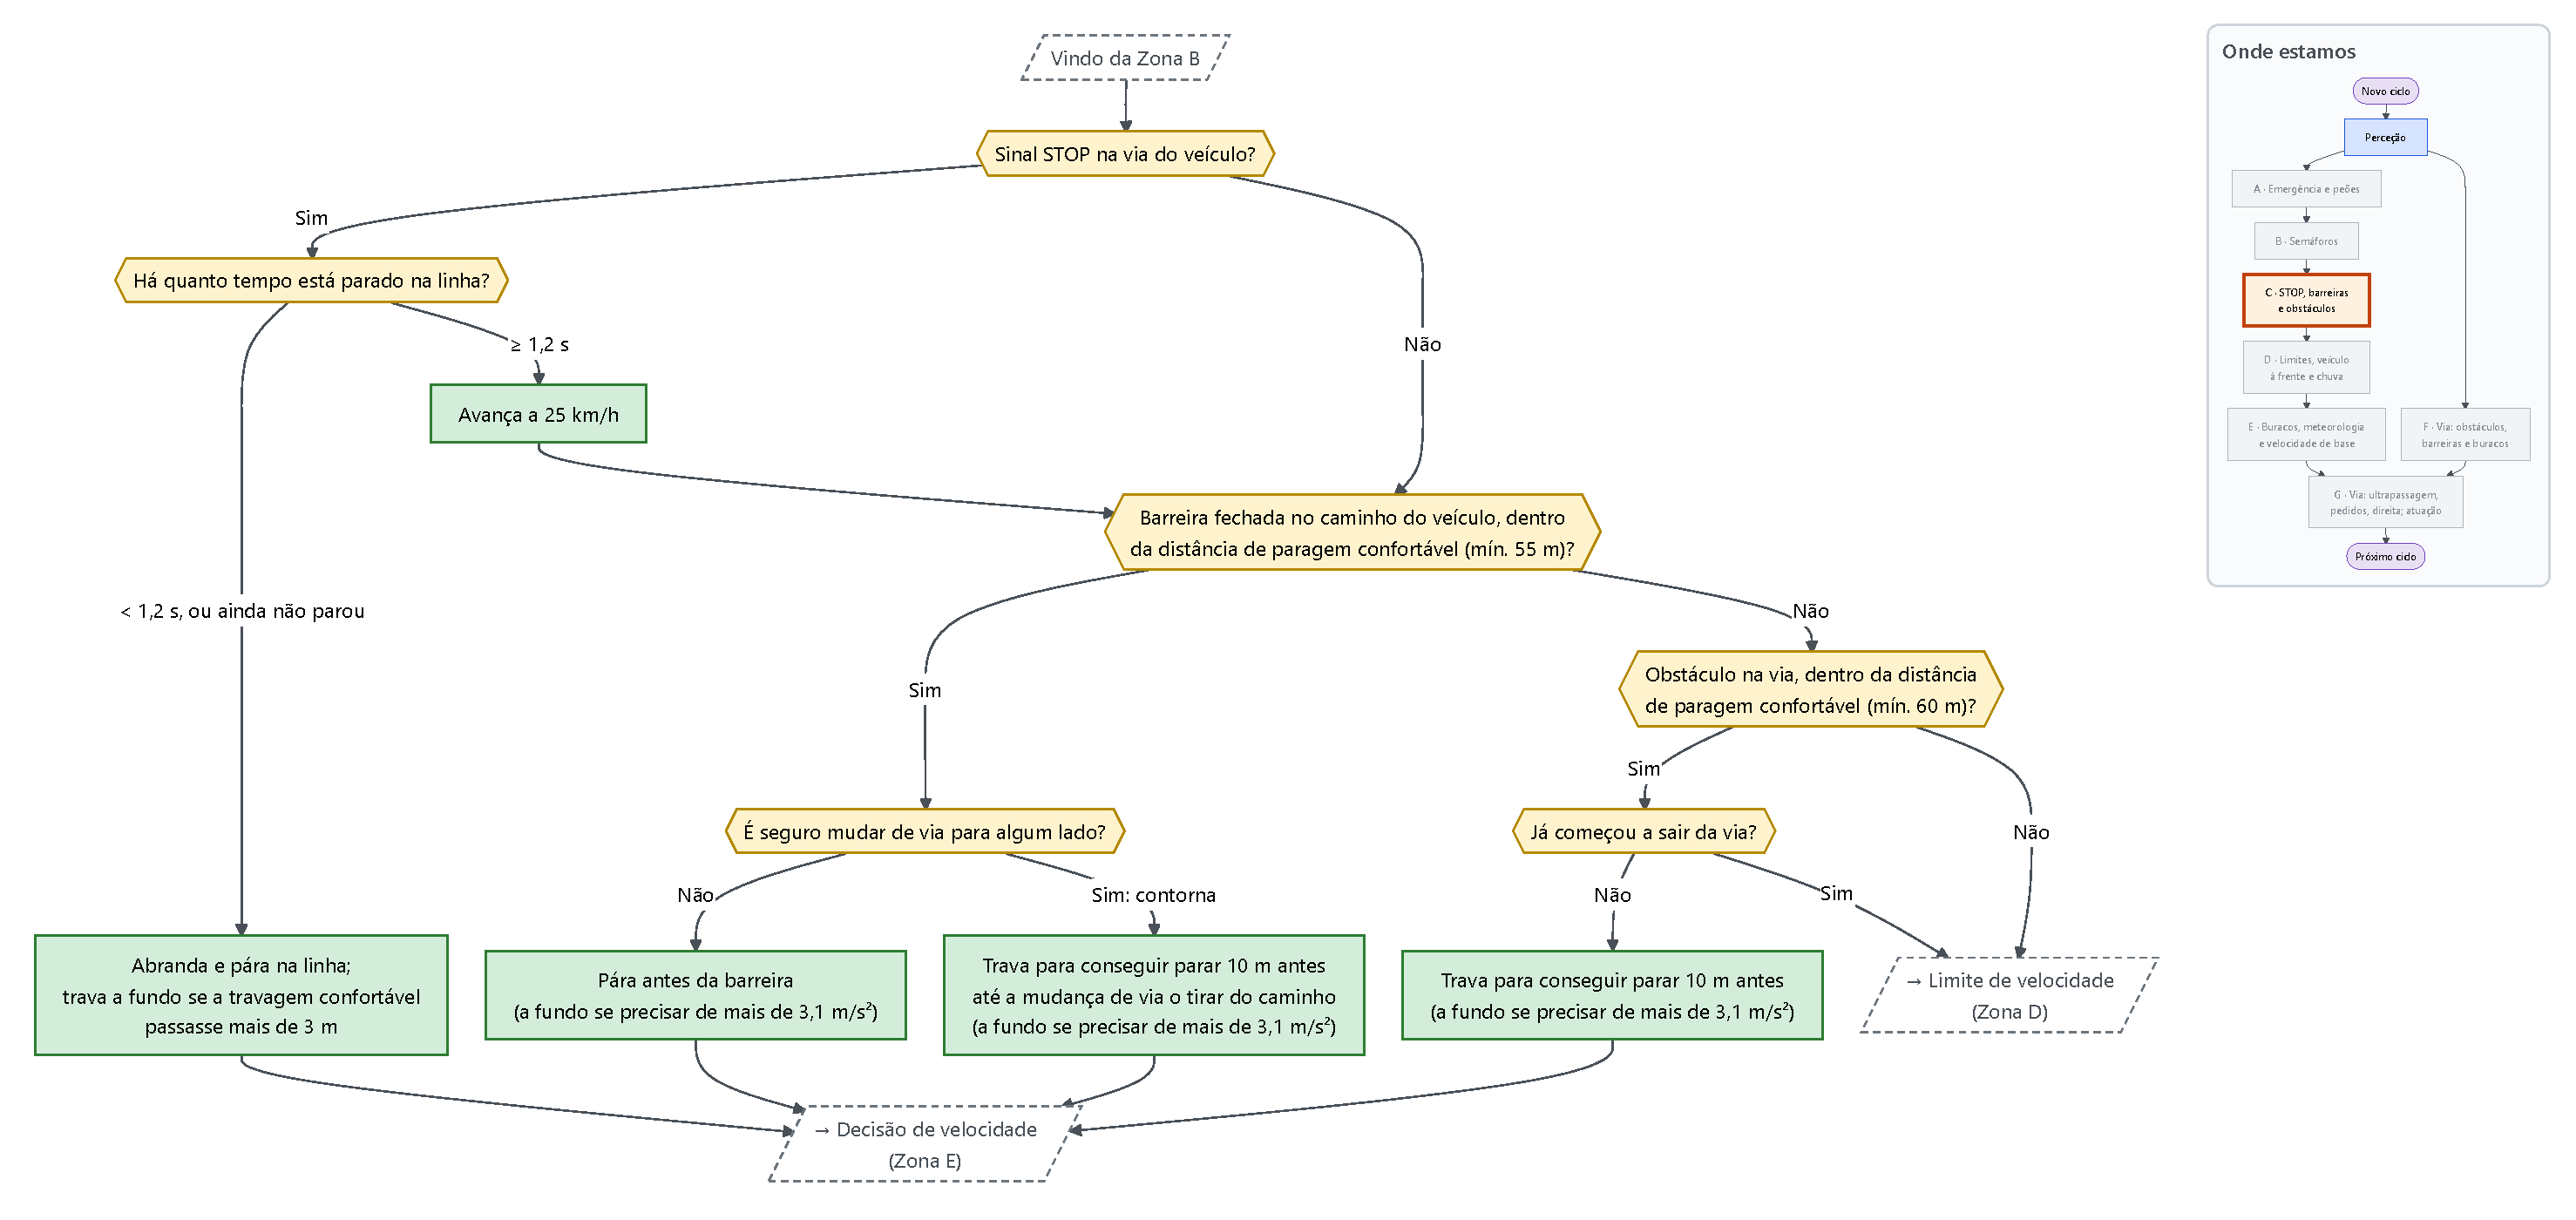
\includegraphics[width=\textheight,height=0.66\textwidth,keepaspectratio]{figuras/fluxograma/zona_C.pdf}
\caption{Zona C: STOP, barreiras e obstáculos}
\label{fig:zonaC}
\end{sidewaysfigure}

\clearpage
\noindent\textbf{Zona D -- Limites, veículo à frente e chuva (\cref{fig:zonaD}).} Esta zona produz
tetos de velocidade (prioridades 50 e 20), que se aplicam todos ao mesmo tempo. O veículo respeita
o limite em vigor e começa a abrandar a tempo de chegar ao sinal seguinte já com o novo limite,
travando a 2,0 m/s². Com um veículo à frente, pára cerca de 12 m atrás se este estiver parado. Se
estiver em movimento, abranda até 3 km/h abaixo dele, acompanha a sua velocidade ou abranda apenas
o necessário, conforme a distância. Com pouca aderência, essa distância duplica. O veículo não
ultrapassa pela direita um veículo mais lento na via da esquerda. Com chuva, duas leituras de TTC
inferiores a 3 s em 2 s levam o veículo a travar até 15 km/h.

\begin{figure}[H]
\centering
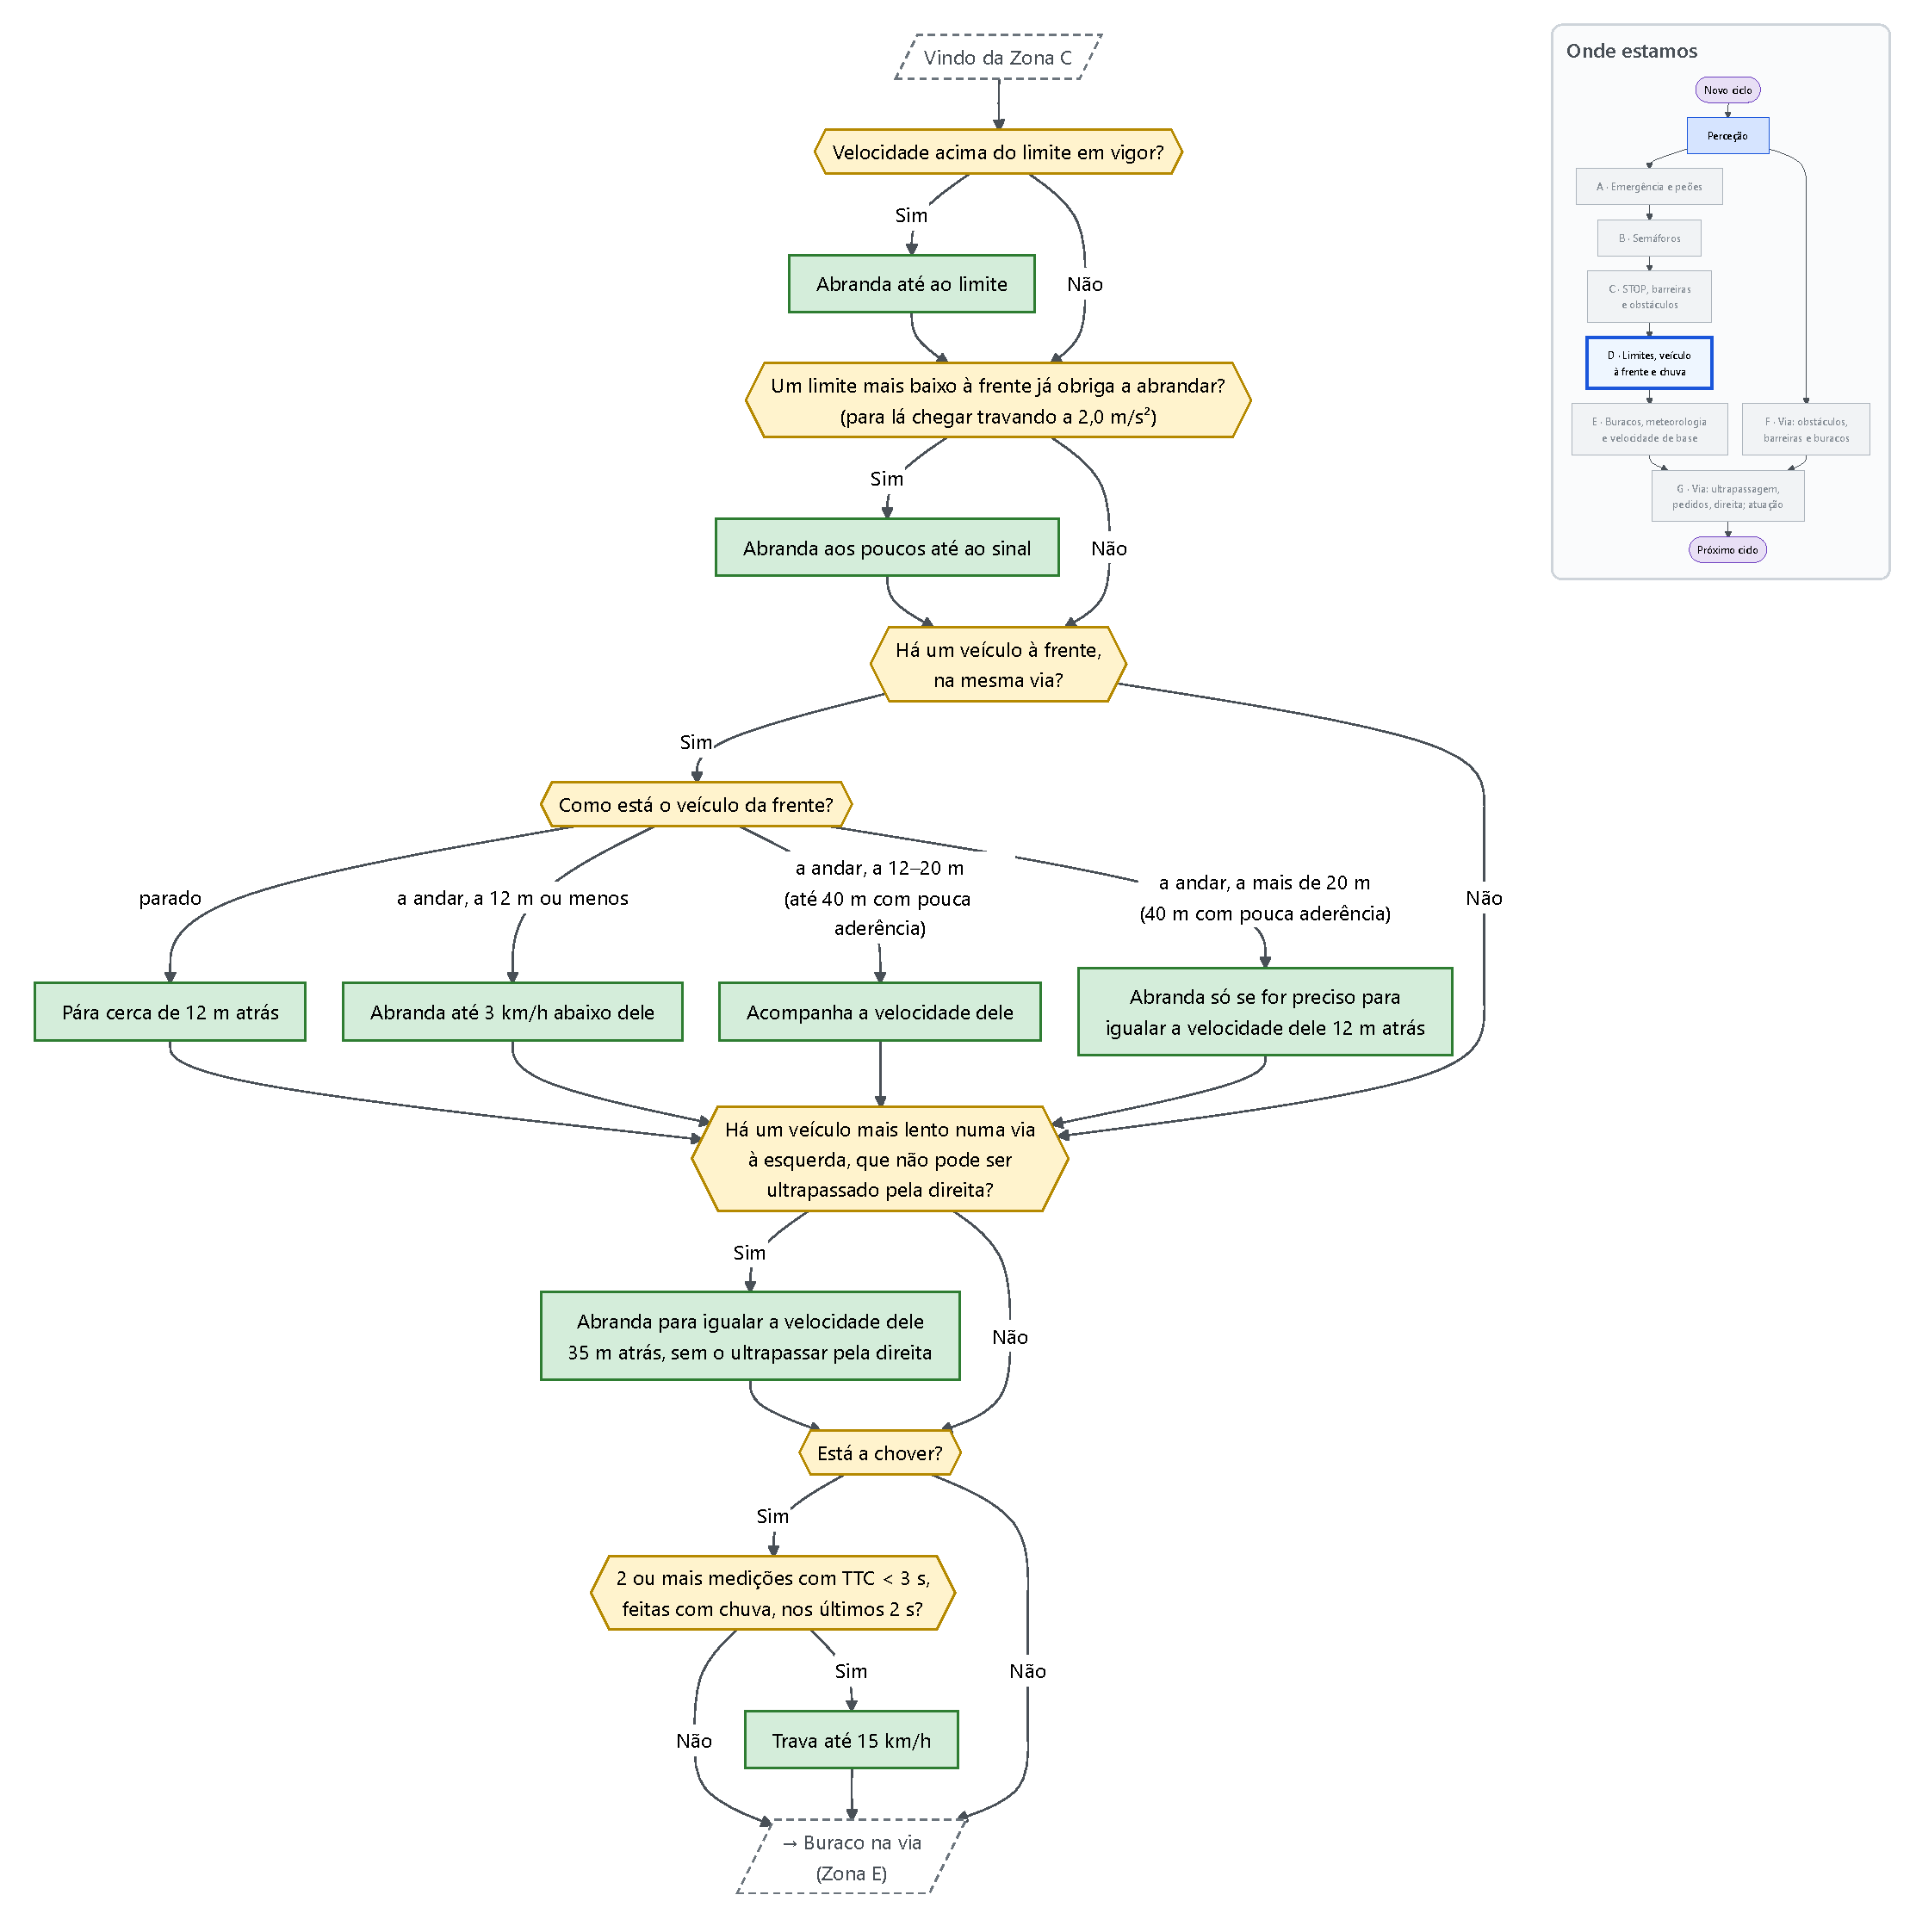
\includegraphics[width=\textwidth,height=0.70\textheight,keepaspectratio]{figuras/fluxograma/zona_D.pdf}
\caption{Zona D: limites, veículo à frente e chuva}
\label{fig:zonaD}
\end{figure}

\clearpage
\noindent\textbf{Zona E -- Buracos, meteorologia e velocidade de base (\cref{fig:zonaE}).} Se não
conseguir desviar-se de um buraco, o veículo passa por ele a 30 km/h, e a 20 km/h nos últimos 15 m.
Junto a uma barreira aberta, não passa de 35 km/h. Com chuva, visibilidade reduzida ou pouca
aderência, a lógica difusa calcula uma velocidade máxima recomendada, entre cerca de 25 e pouco
mais de 70 km/h. Só depois de considerados todos os tetos é definida a velocidade de base: arrancar
após uma paragem, acelerar a pedido, manter o limite do sinal ou retomar a velocidade de cruzeiro.
Se nenhuma regra se aplicar, a fase de recurso mantém a velocidade. Por fim, vale a velocidade mais
baixa entre a de base e todos os tetos encontrados, pelo que o veículo nunca ultrapassa o limite
legal.

\begin{figure}[H]
\centering
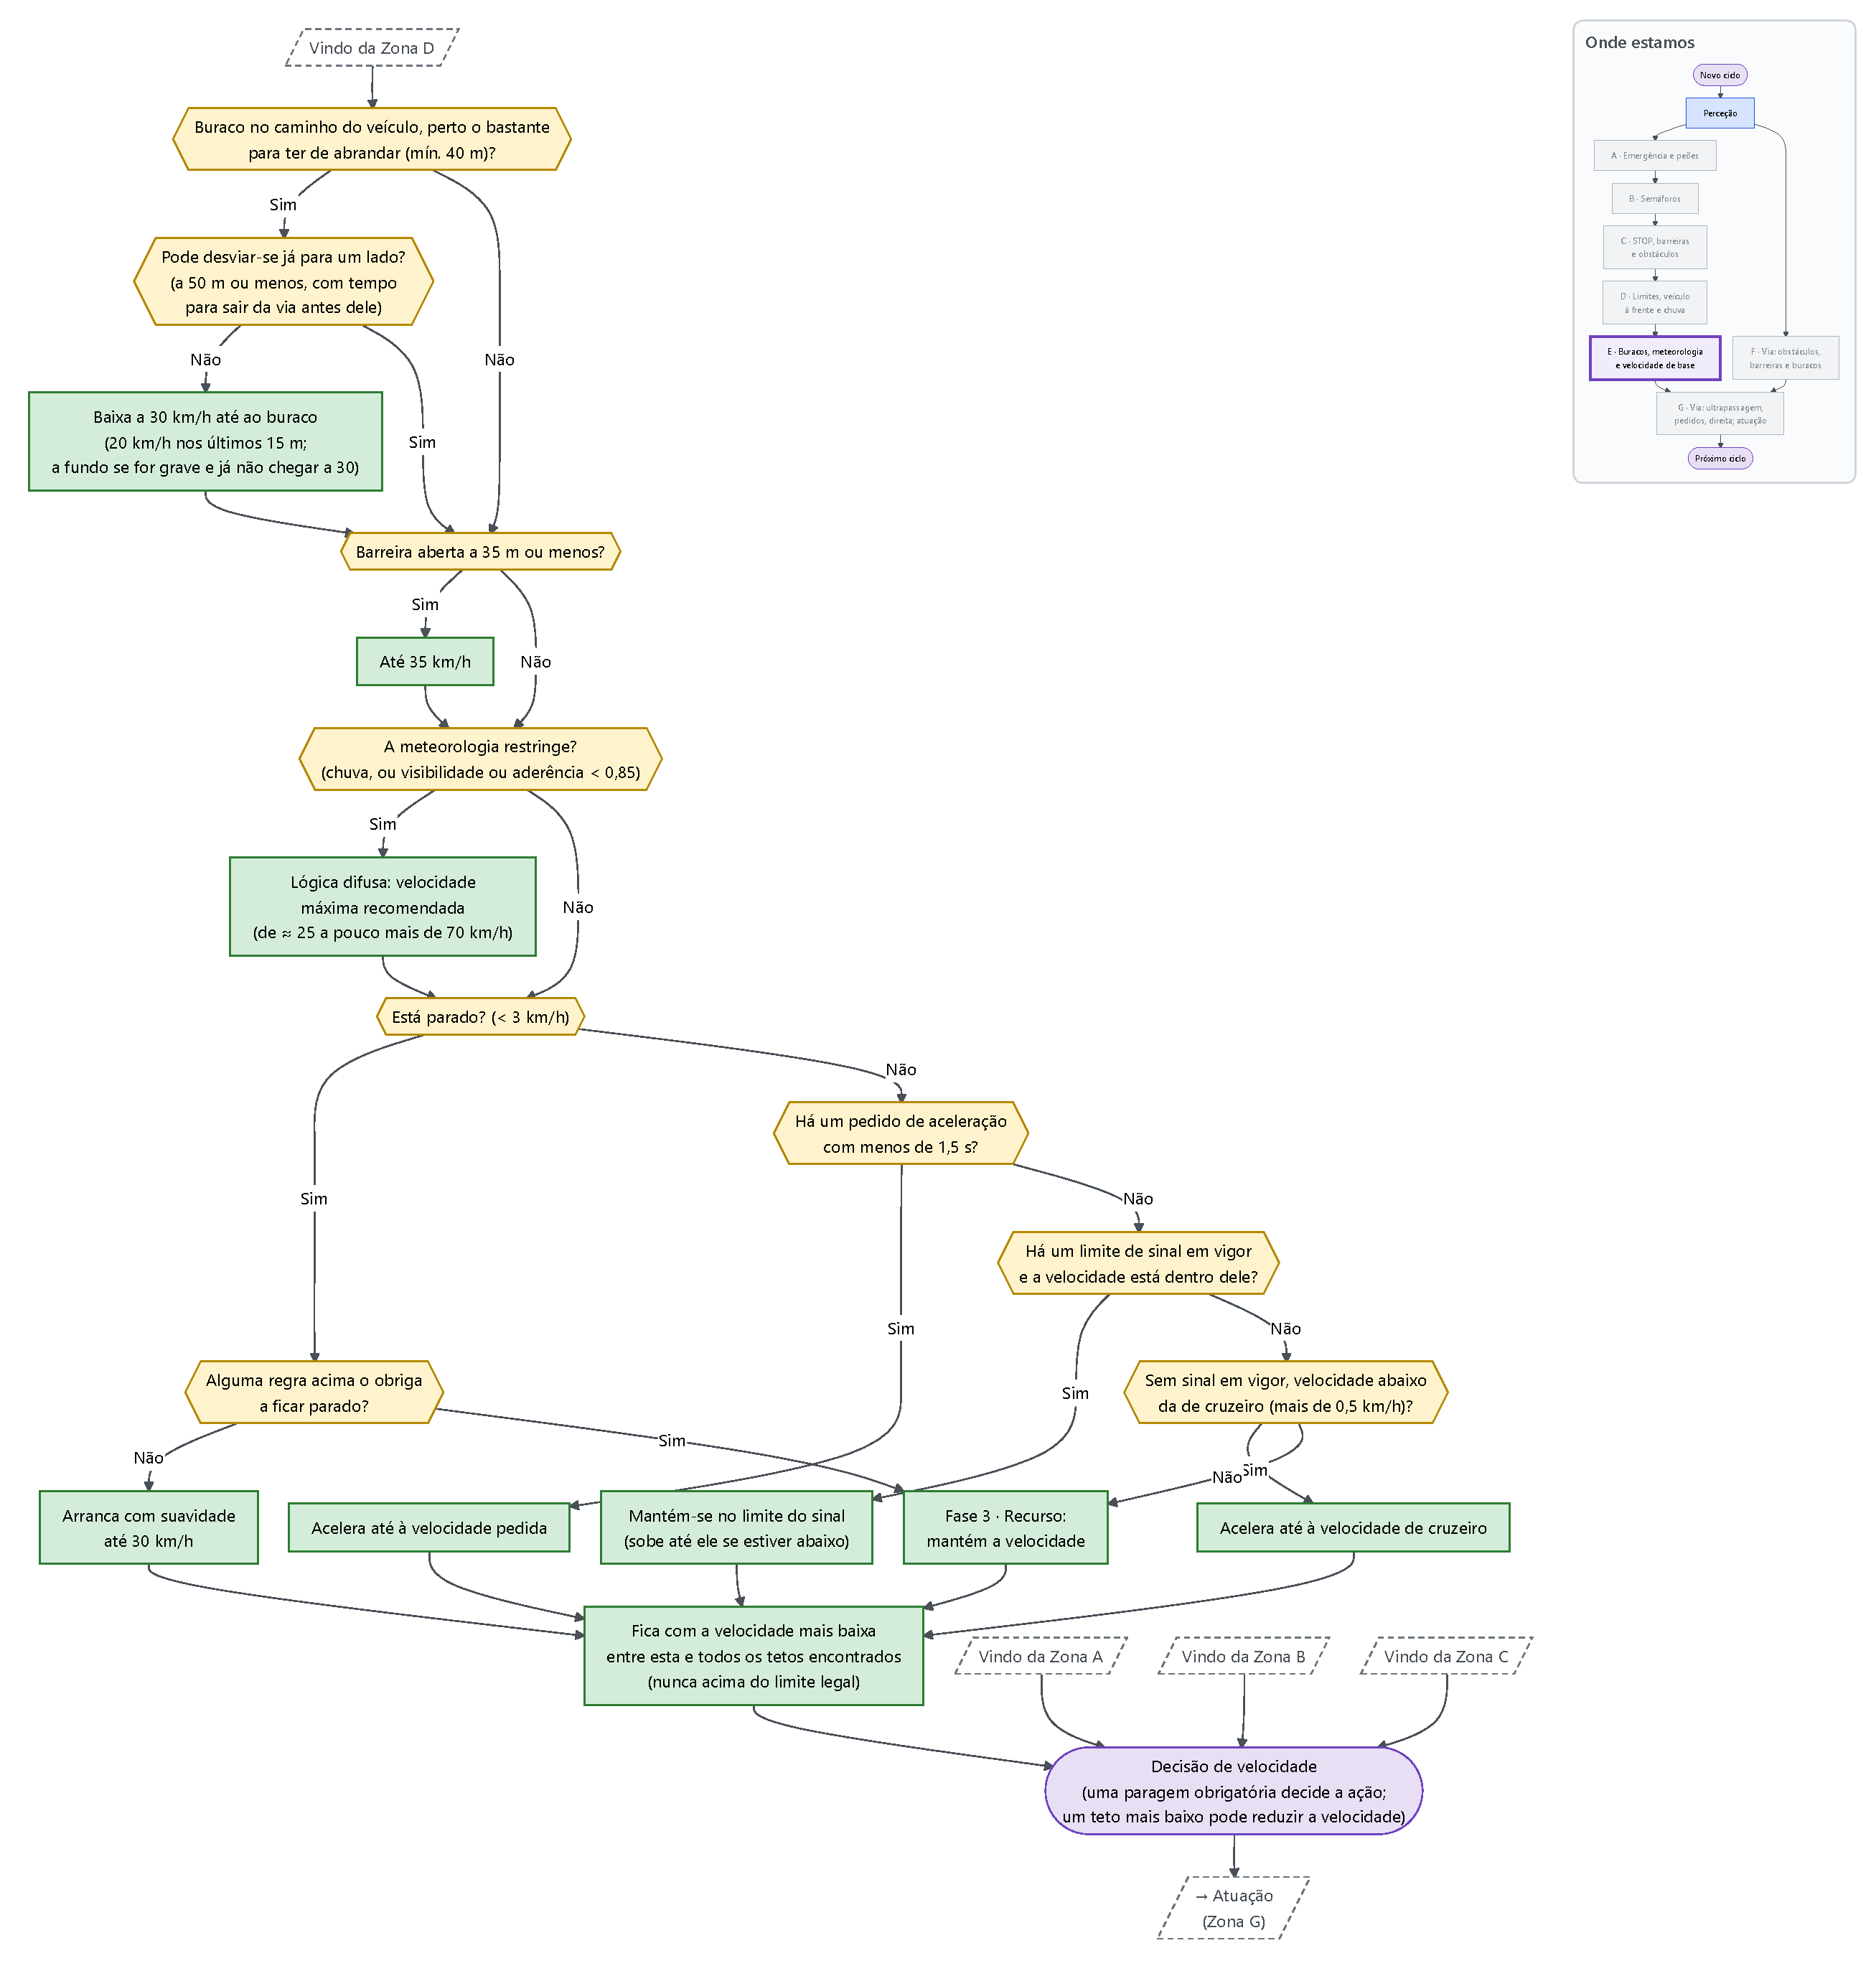
\includegraphics[width=\textwidth,height=0.70\textheight,keepaspectratio]{figuras/fluxograma/zona_E.pdf}
\caption{Zona E: buracos, meteorologia e velocidade de base}
\label{fig:zonaE}
\end{figure}

\clearpage
\begin{sidewaysfigure}
\begin{minipage}{\linewidth}
\noindent\textbf{Zona F -- Via: obstáculos, barreiras e buracos (\cref{fig:zonaF}).} O canal de via
começa por confirmar se uma emergência ou paragem obrigatória está a travar o veículo. Se estiver,
o veículo mantém a via, o que garante que nenhuma manobra compete com uma travagem crítica. Uma
mudança de via já iniciada é sempre concluída. Perante um obstáculo, uma barreira fechada ou um
buraco na via, o veículo contorna-o se for seguro mudar de via e se ainda conseguir sair da via
antes de lá chegar. Caso contrário, mantém a via e o canal de velocidade trata da paragem ou da
passagem lenta.
\end{minipage}

\vspace{4mm}
\centering
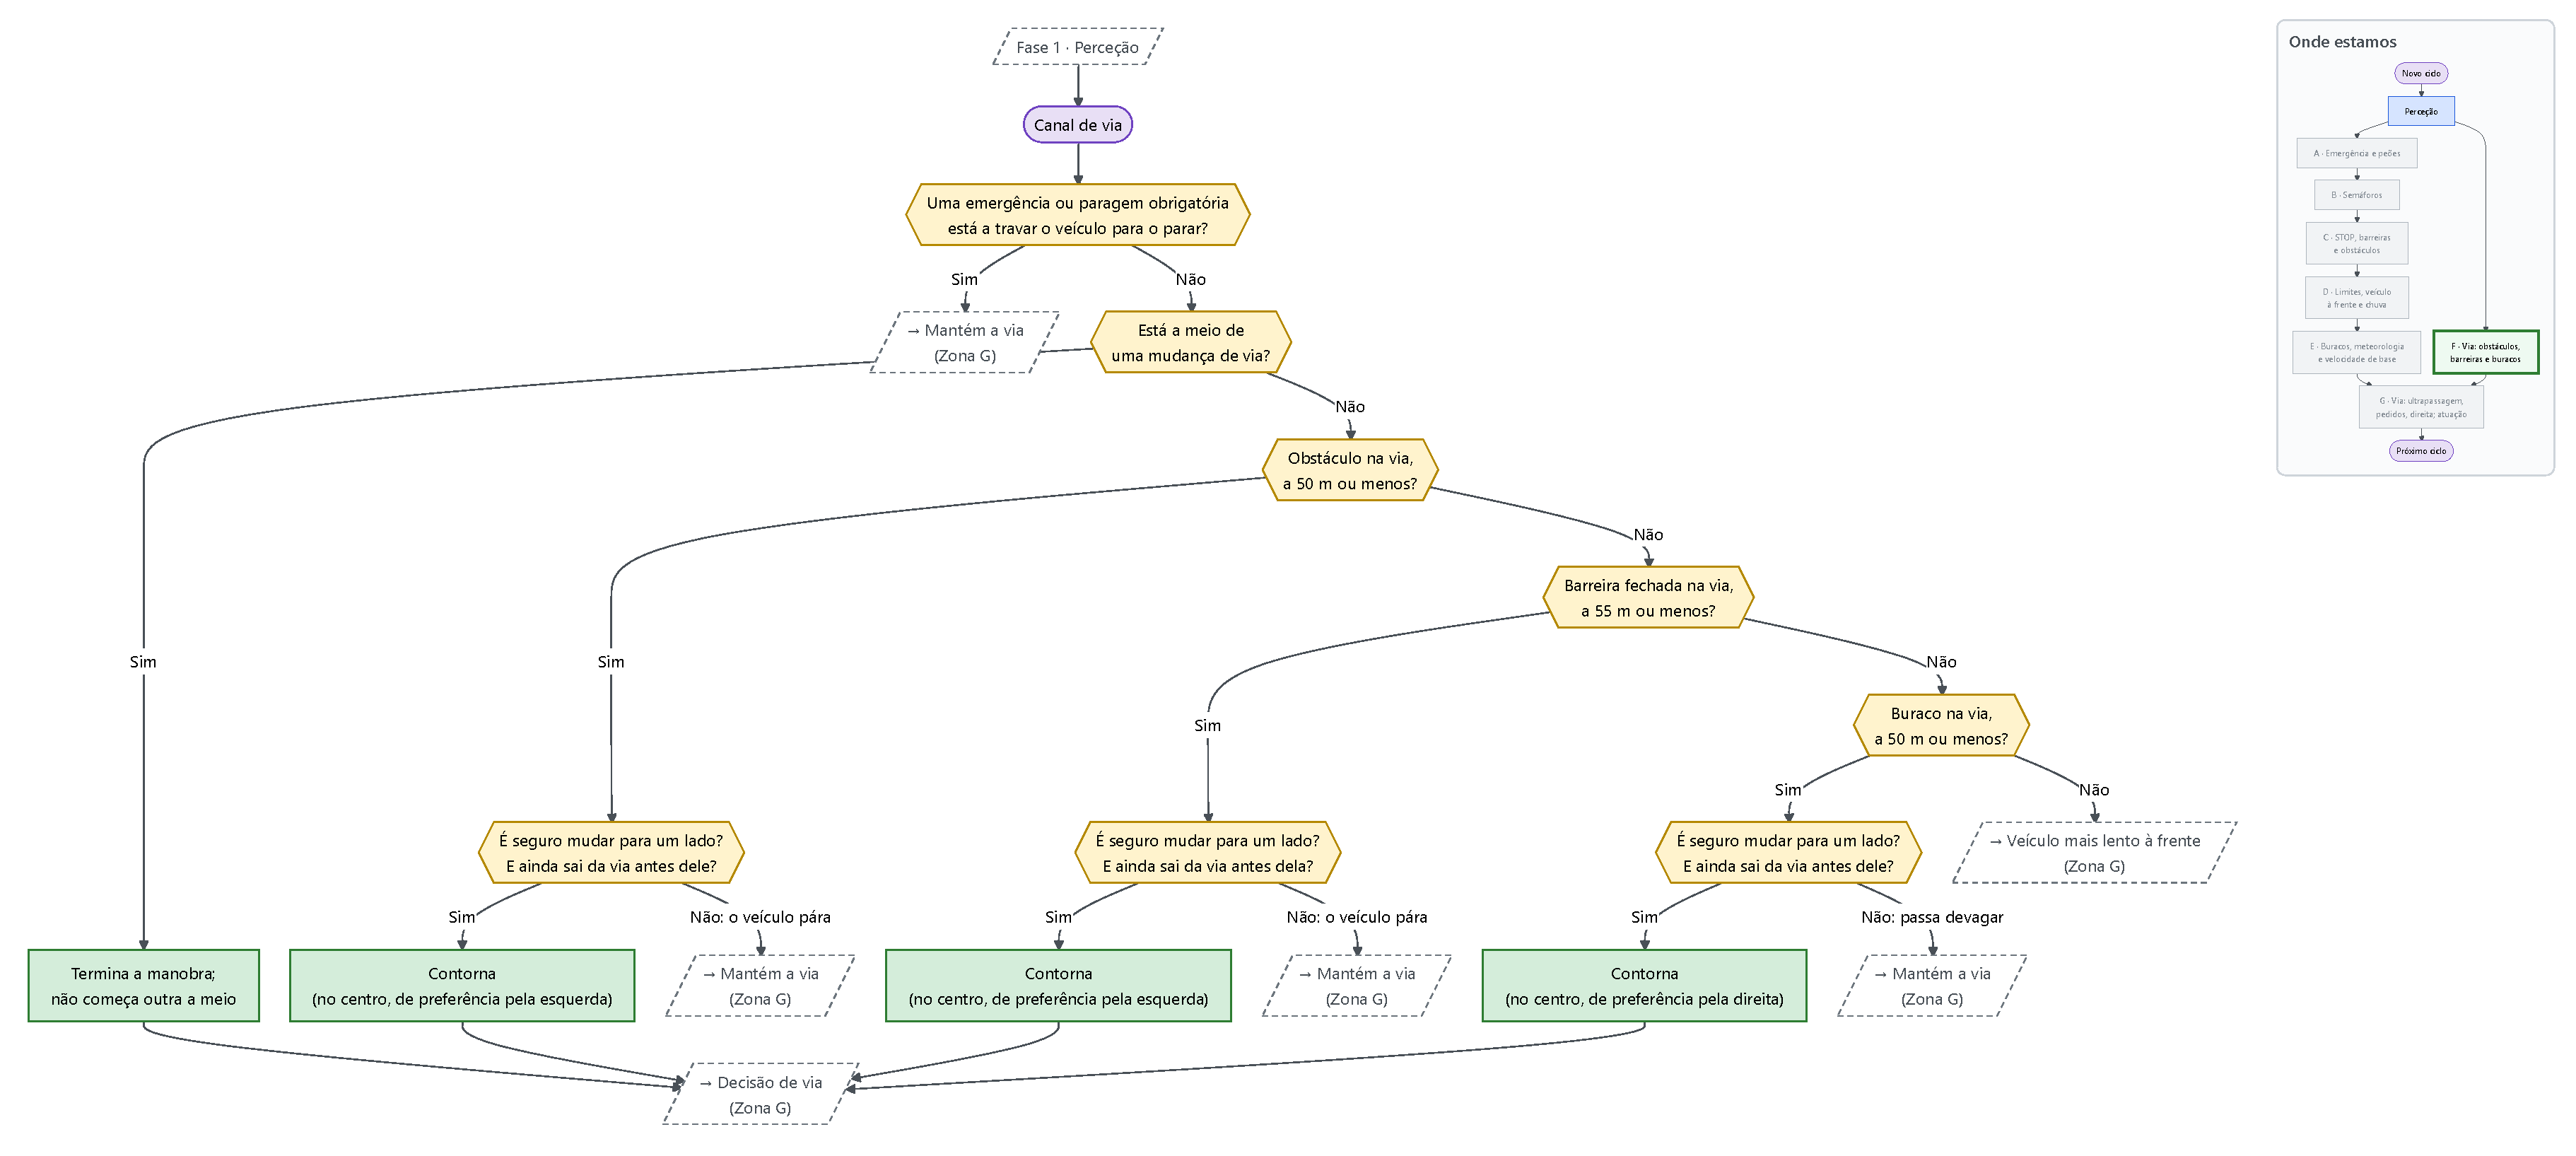
\includegraphics[width=\textheight,height=0.64\textwidth,keepaspectratio]{figuras/fluxograma/zona_F.pdf}
\caption{Zona F: canal de via perante obstáculos, barreiras e buracos}
\label{fig:zonaF}
\end{sidewaysfigure}

\begin{sidewaysfigure}
\begin{minipage}{\linewidth}
\noindent\textbf{Zona G -- Ultrapassagem, pedidos, regresso à direita e atuação
(\cref{fig:zonaG}).} Atrás de um veículo mais lento, o veículo ultrapassa apenas pela esquerda. Se
estiver preso atrás de trânsito lento em todas as vias há pelo menos 3 s, desiste e regressa à
direita. Um pedido externo de mudança de via só é aceite se a mudança for segura; se não for, é
recusado e a explicação indica qual das condições falhou. Sem outro motivo para ficar, o veículo
regressa à via da direita, uma via de cada vez, como determina o Código da Estrada. As decisões de
velocidade e de via juntam-se na atuação. Antes de iniciar uma mudança de via, o atuador volta a
confirmar no mundo que a via de destino está livre e que não há linha contínua. Se alguma destas
condições falhar, cancela a manobra e abranda 10 km/h. Por fim, ajusta a velocidade com suavidade e
começa o ciclo seguinte.
\end{minipage}

\vspace{4mm}
\centering
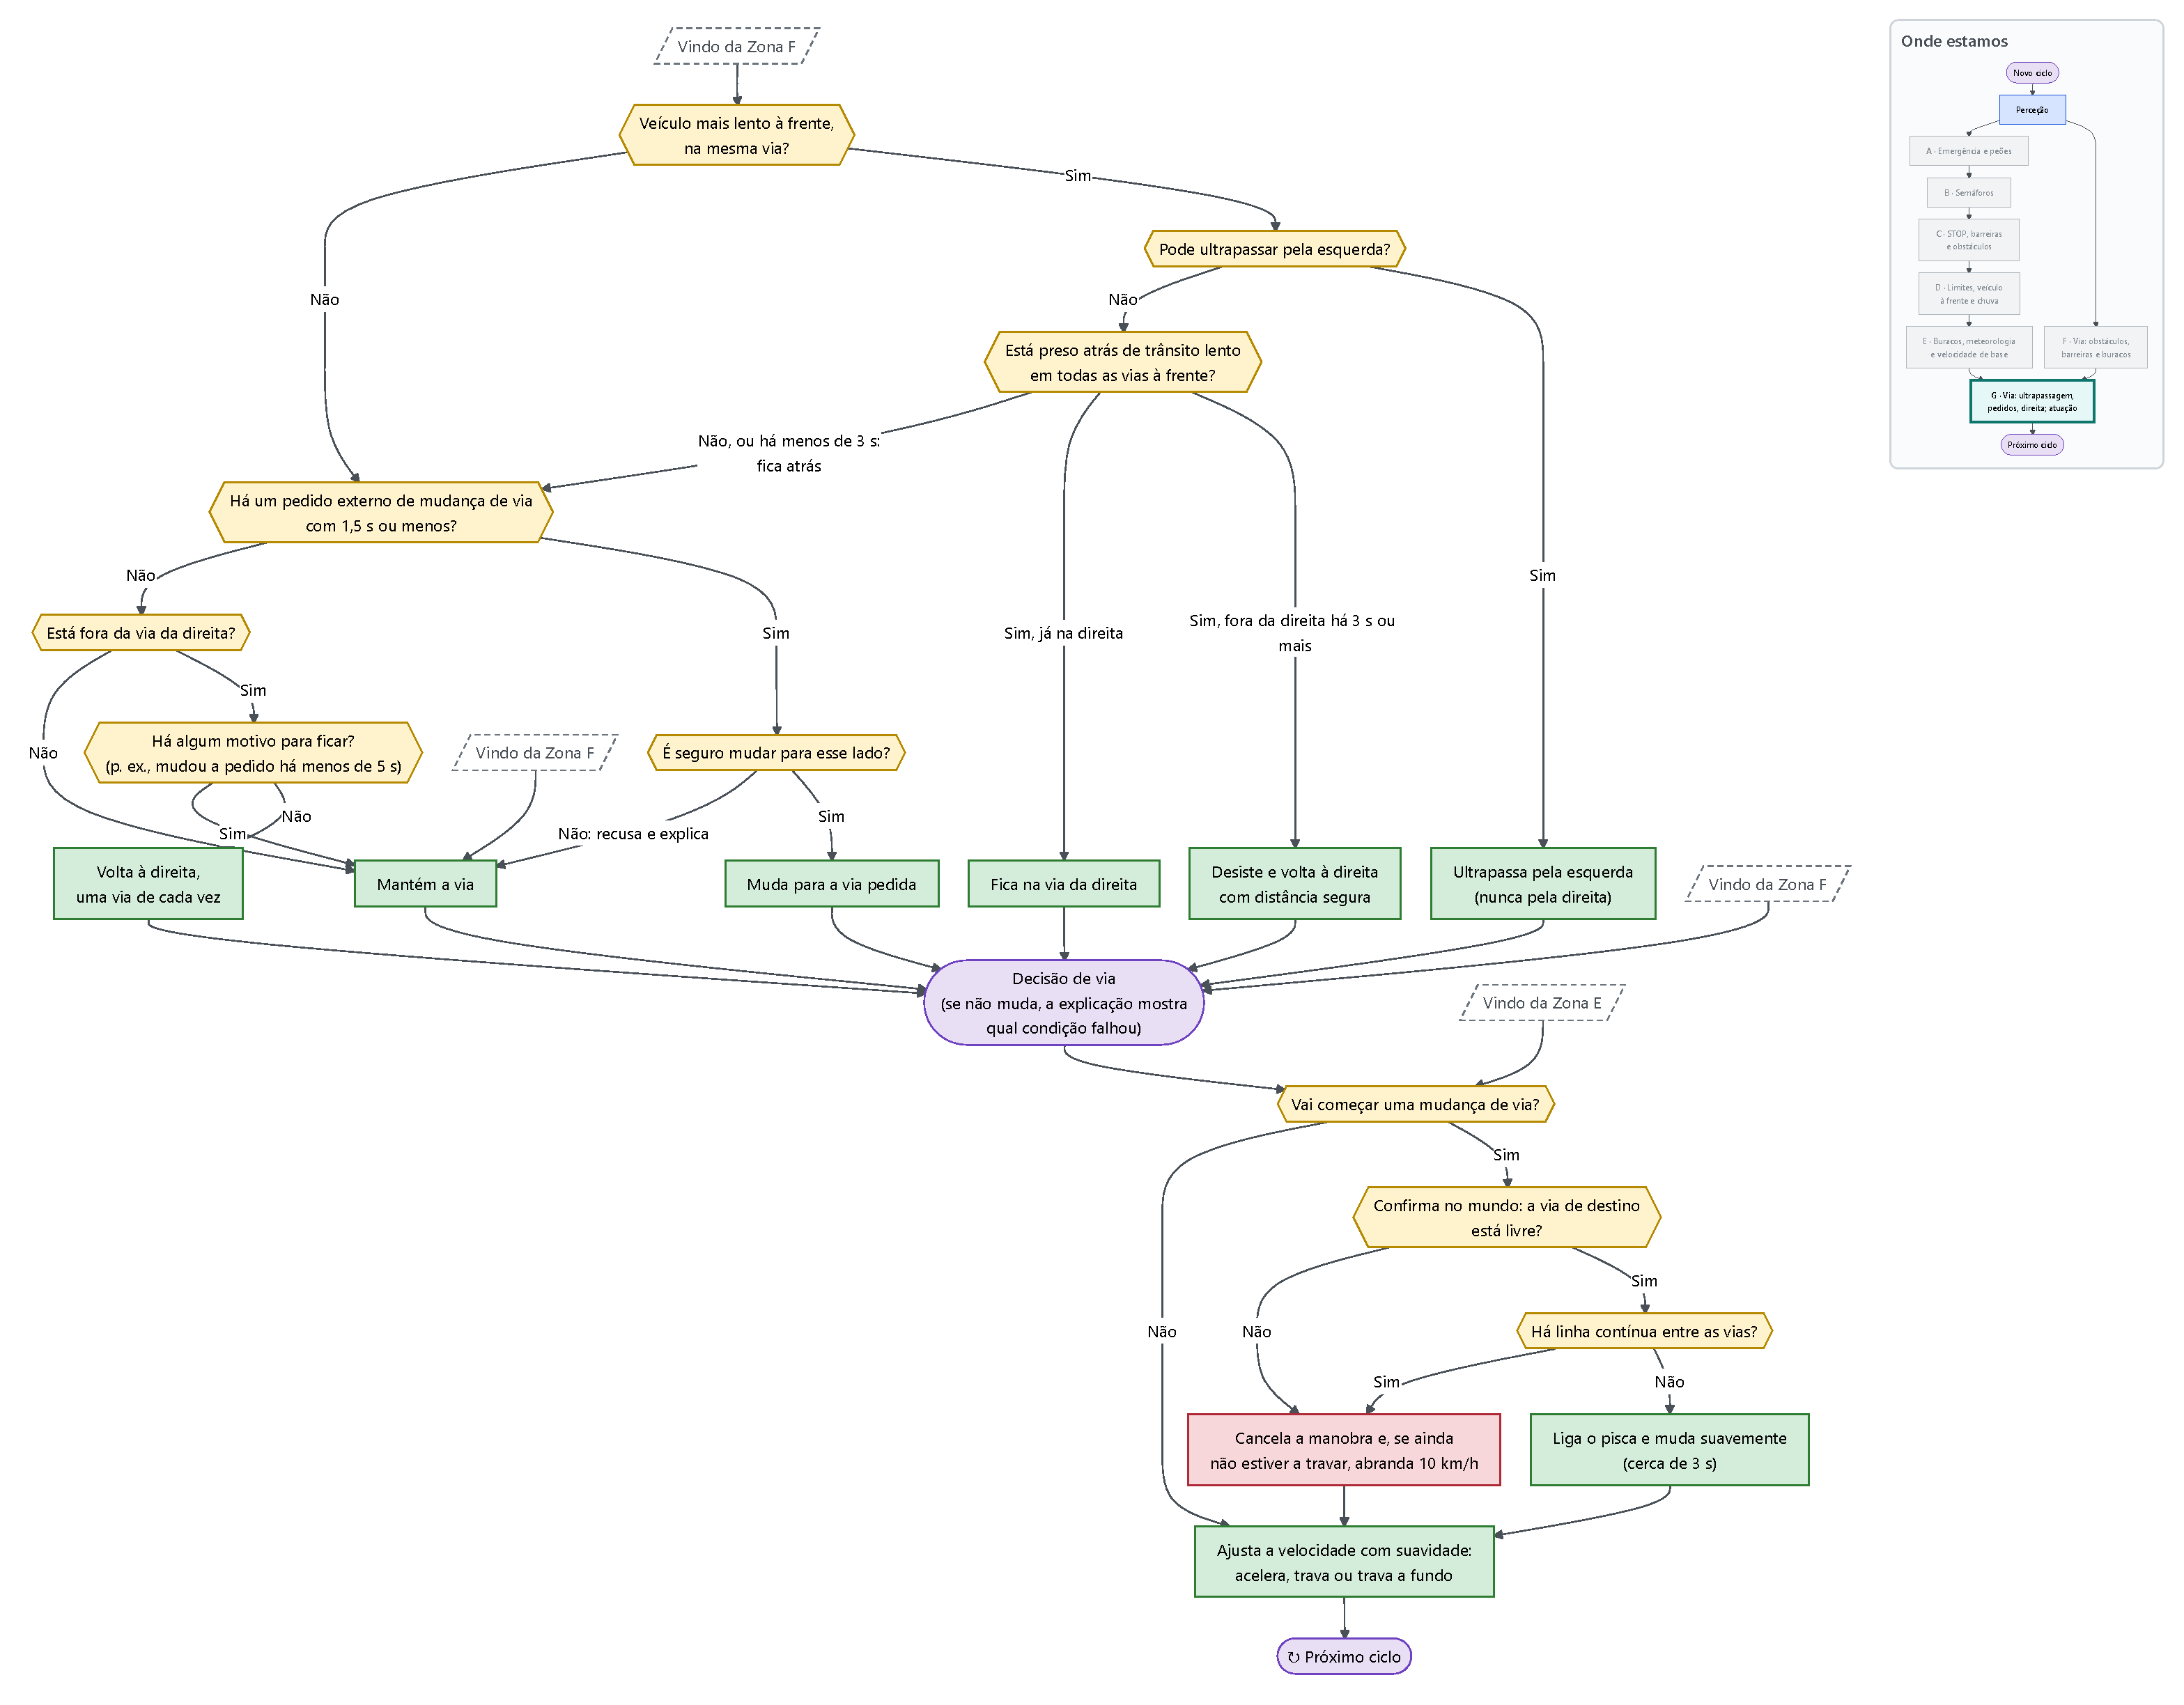
\includegraphics[width=\textheight,height=0.58\textwidth,keepaspectratio]{figuras/fluxograma/zona_G.pdf}
\caption{Zona G: ultrapassagem, pedidos, regresso à direita e atuação}
\label{fig:zonaG}
\end{sidewaysfigure}

\clearpage

\section{Explicação da decisão}\label{sec:explicacao}

Cada decisão pode ser explicada em três dimensões complementares (Figura 15), todas implementadas e visíveis na interface.

\begin{figure}[htbp]
\centering
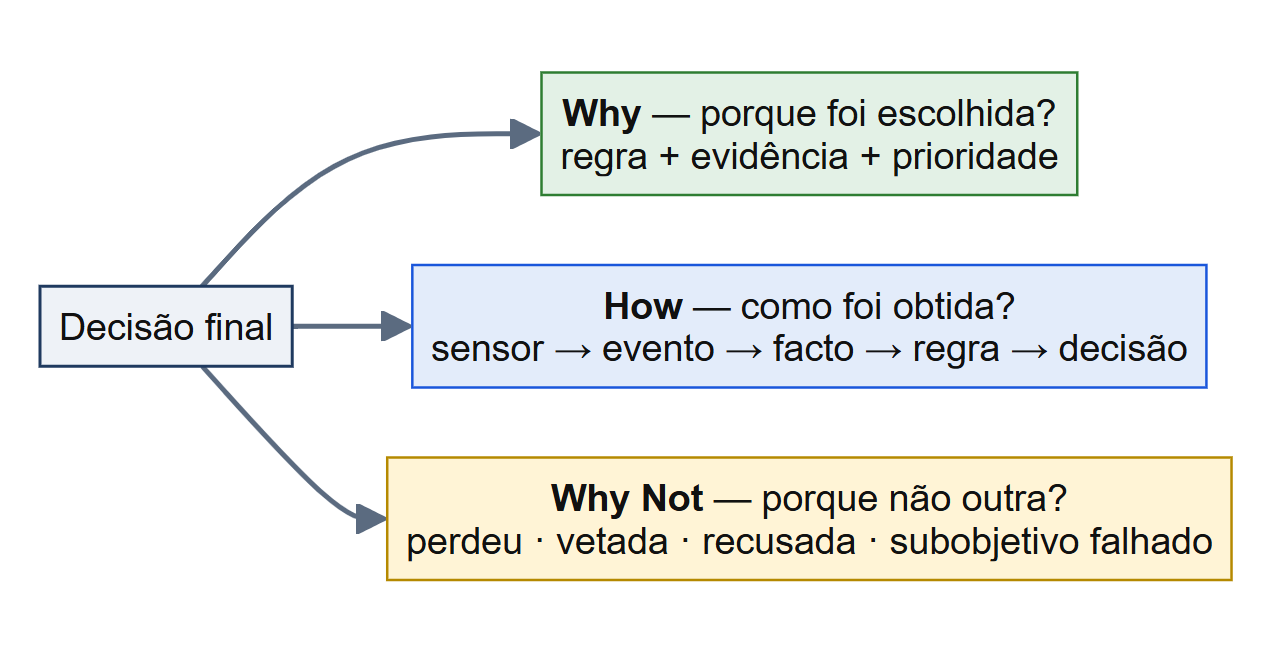
\includegraphics[width=0.62\textwidth]{figuras/explicacao.png}
\caption{Três dimensões de explicação}
\label{fig:explicacao}
\end{figure}

\begin{itemize}
  \item \textbf{\ing{Why}.} A decisão guarda, por canal, a regra que a originou, a razão, a
        evidência (os valores dos factos usados), o risco e a prioridade.
  \item \emph{\textbf{How}}. A linha temporal regista, com instante, cada inserção, atualização e remoção de factos e cada regra disparada, o que permite reconstruir o percurso sensor → evento → facto → regra → decisão. O inspetor da memória de trabalho mostra os factos ativos e, na explicação da viagem, o How percorre as perguntas das Figuras 5 e 6 e mostra o ramo seguido em cada uma.
  \item \textbf{\ing{Why Not}.} Todas as propostas do ciclo ficam guardadas com o seu destino:
        venceu, perdeu para outra (\cod{LOST\_TO}), foi anulada por uma paragem ou emergência
        (\cod{VETOED\_BY}), teve a velocidade limitada por um teto (\cod{CAPPED}) ou foi recusada
        pelo atuador (\cod{REJECTED\_BY}). Quando uma mudança de via nem chega a ser proposta, o
        sistema mostra qual dos subobjetivos de segurança falhou (manobra em curso, linha
        contínua, via ocupada ou falta de espaço para seguir o veículo da frente).
\end{itemize}

Como recomendou o perito, as explicações são o resultado das próprias regras: o texto apresentado
é a razão e a evidência registadas pela regra que disparou, e não uma descrição escrita à parte. Ao
terminar uma viagem (STOP), a sessão é gravada em JSON e cada decisão pode ser questionada depois, a
partir do ciclo gravado, sem reavaliar nada.

O capítulo seguinte mostra como este processo está implementado e como pode ser acompanhado em
tempo real.
